% Institute of Computer Science thesis template
% authors: Sven Laur, Liina Kamm
% last change Tõnu Tamme 09.05.2017
%--
% Compilation instructions:
% 1. Choose main language on line 55-56 (English or Estonian)
% 2. Compile 1-3 times to get refences right
% pdflatex bachelors-thesis-template
% bibtex bachelors-thesis-template
%--
% Please use references like this:
% <text> <non-breaking-space> <cite/ref-command> <punctuation>
% This is an example~\cite{example}.

\documentclass[12pt]{article}

% A package for setting layout and margins for your thesis 
\usepackage[a4paper]{geometry}

%%=== A4 page setup ===
%\setlength{\paperwidth}{21.0cm} 
%\setlength{\paperheight}{29.7cm}
%\setlength{\textwidth}{16cm}
%\setlength{\textheight}{25cm}


% When you write in Estonian then you want to use text with right character set
% By default LaTeX does not know what to do with õäöu letters. You have to specify
% a correct input and font encoding. For that you have to Google the Web     
%
% For TexShop under MacOS X. The right lines are 
%\usepackage[applemac]{inputenc}
%\usepackage[T1]{fontenc} %Absolutely critical for *hyphenation* of words with non-ASCII letters.
%
% For Windows and Linux the right magic lines are   
% \usepackage[latin1]{inputenc}
% \usepackage[latin5]{inputenc}
%%\usepackage[utf8]{inputenc} %Package inputenc Error: Unicode char ´ (U+B4) not set up for use with LaTeX
\usepackage[utf8x]{inputenc}
\usepackage[T1]{fontenc} %Absolutely critical for *hyphenation* of words with non-ASCII letters.

% Typeset text in Times Roman instead of Computer Modern (EC)
\usepackage{times}

% Suggested packages:
\usepackage{microtype}  %towards typographic perfection...
\usepackage{inconsolata} %nicer font for code listings. (Use \ttfamily for lstinline bastype)


% Use package babel for English or Estonian 
% If you use Estonian make sure that Estonian hyphenation is installed 
% - hypen-estonian or eehyp packages
%
%===Choose the main language in thesis
\usepackage[estonian, english]{babel} %the thesis is in English 
%\usepackage[english, estonian]{babel} %the thesis is in Estonian


% Change Babel document elements 
\addto\captionsestonian{%
  \renewcommand{\refname}{Viidatud kirjandus}%
  \renewcommand{\appendixname}{Lisad}%
}


% If you have problems with Estonian keywords in the bibliography
%\usepackage{biblatex}
%\usepackage[backend=biber]{biblatex}
%\usepackage[style=alphabetic]{biblatex}
% plain --> \usepackage[style=numeric]{biblatex}
% abbrv --> \usepackage[style=numeric,firstinits=true]{biblatex}
% unsrt --> \usepackage[style=numeric,sorting=none]{biblatex}
% alpha --> \usepackage[style=alphabetic]{biblatex}
%\DefineBibliographyStrings{estonian}{and={ja}}
%\addbibresource{bachelor-thesis.bib}


% General packages for math in general, theorems and symbols 
% Read ftp://ftp.ams.org/ams/doc/amsmath/short-math-guide.pdf for further information
\usepackage{amsmath} 
\usepackage{amsthm}
\usepackage{amssymb}

% Optional calligraphic fonts    
% \usepackage[mathscr]{eucal}

% Print a dot instead of colon in table or figure captions
\usepackage[labelsep=period]{caption}

% Packages for building tables and tabulars 
\usepackage{array}
\usepackage{tabu}   % Wide lines in tables
\usepackage{xspace} % Non-eatable spaces in macros

% Including graphical images and setting the figure directory
\usepackage{graphicx}
\graphicspath{{fig/}}

% Packages for getting clickable links in PDF file
%\usepackage{hyperref}
\usepackage[hidelinks]{hyperref} %hide red (blue,green) boxes around links
\usepackage[all]{hypcap}


% Packages for defining colourful text together with some colours
\usepackage{color}
\usepackage{xcolor} 
\definecolor{dkgreen}{rgb}{0,0.6,0}
\definecolor{gray}{rgb}{0.5,0.5,0.5}
\definecolor{mauve}{rgb}{0.58,0,0.82}


% Standard package for drawing algorithms
% Since the thesis in article format we must define \chapter for
% the package algorithm2e (otherwise obscure errors occur) 
\let\chapter\section
\usepackage[ruled, vlined, linesnumbered]{algorithm2e}

% Fix a  set of keywords which you use inside algorithms
\SetKw{True}{true}
\SetKw{False}{false}
\SetKwData{typeInt}{Int}
\SetKwData{typeRat}{Rat}
\SetKwData{Defined}{Defined}
\SetKwFunction{parseStatement}{parseStatement}


% Nice todo notes
\usepackage{todonotes}

% comments and verbatim text (code)
\usepackage{verbatim}


% Proper way to create coloured code listings
\usepackage{listings}
\lstset{ 
  %language=python,                % the language of the code
  %language=C++,
  language=Java,
  basicstyle=\footnotesize,        % the size of the fonts that are used for the code
  %numbers=left,                   % where to put the line-numbers
  %numberstyle=\footnotesize,      % the size of the fonts that are used for the line-numbers
  numberstyle=\tiny\color{gray}, 
  stepnumber=1,                    % the step between two line-numbers. If it's 1, each line 
                                   % will be numbered
  numbersep=5pt,                   % how far the line-numbers are from the code
  backgroundcolor=\color{white},   % choose the background color. You must add \usepackage{color}
  showspaces=false,                % show spaces adding particular underscores
  showstringspaces=false,          % underline spaces within strings
  showtabs=false,                  % show tabs within strings adding particular underscores
  frame = lines,
  %frame=single,                   % adds a frame around the code
  rulecolor=\color{black},		   % if not set, the frame-color may be changed on line-breaks within 
                                   % not-black text (e.g. commens (green here))
  tabsize=2,                       % sets default tabsize to 2 spaces
  captionpos=b,                    % sets the caption-position to bottom
  breaklines=true,                 % sets automatic line breaking
  breakatwhitespace=false,         % sets if automatic breaks should only happen at whitespace
  %title=\lstname,                 % show the filename of files included with \lstinputlisting;
                                   % also try caption instead of title
  keywordstyle=\color{blue},       % keyword style
  commentstyle=\color{dkgreen},    % comment style
  stringstyle=\color{mauve},       % string literal style
  escapeinside={\%*}{*)},          % if you want to add a comment within your code
  morekeywords={*,game, fun}       % if you want to add more keywords to the set
}

\renewcommand{\lstlistingname}{Code Snippet}
\renewcommand{\lstlistlistingname}{List of \lstlistingname s}


% Obscure packages to write logic formulae and program semantics
% Unless you do a bachelor thesis on program semantics or static code analysis you do not need that
% http://logicmatters.net/resources/ndexamples/proofsty3.html <= writing type rules => use semantic::inference
% ftp://tug.ctan.org/tex-archive/macros/latex/contrib/semantic/semantic.pdf
\usepackage{proof}
\usepackage{semantic} 
\setlength{\inferLineSkip}{4pt}
\def\predicatebegin #1\predicateend{$\Gamma \vdash #1$}

% If you really want to draw figures in LaTeX use packages tikz or pstricks
% However, getting a corresponding illustrations is really painful  


% Define your favorite macros that you use inside the thesis 
% Name followed by non-removable space
\newcommand{\proveit}{ProveIt\xspace}

% Macros that make sure that the math mode is set
\newcommand{\typeF}[1] {\ensuremath{\mathsf{type_{#1}}}\xspace}
\newcommand{\opDiv}{\ensuremath{\backslash \mathsf{div}}\xspace} 

% Nice Todo box
\newcommand{\TODO}{\todo[inline]}

% A way to define theorems and lemmata
\newtheorem{theorem}{Theorem}



%%% BEGIN DOCUMENT
\begin{document}

%===BEGIN TITLE PAGE
\thispagestyle{empty}
\begin{center}

\iflanguage{english}{%
\large
UNIVERSITY OF TARTU\\%[2mm]
Institute of Computer Science\\
Security and Mobile Computing Curriculum\\%[2mm]
}{%
TARTU ÜLIKOOL\\
Arvutiteaduse instituut\\
Informaatika õppekava\\%[2mm]
}%\iflanguage

%\vspace*{\stretch{5}}
\vspace{25mm}

\Large Jes\'{u}s Antonio Soto Vel\'{a}zquez

\vspace{4mm}

\huge Securing openHAB Smart Home through User Authentication and Authorization \\

%\vspace*{\stretch{7}}
\vspace{20mm}

\iflanguage{english}{%
\Large Master's Thesis (30 ECTS)
}{%
\Large Bakalaureusetöö (9 EAP)
}%\iflanguage

\end{center}

\vspace{2mm}

\begin{flushright}
 {
 \setlength{\extrarowheight}{5pt}
 \begin{tabular}{r l} 
  \sffamily \iflanguage{english}{Supervisor}{Juhendaja}: & \sffamily Satish Narayana Srirama, PhD \\
  \sffamily \iflanguage{english}{Supervisor}{Juhendaja}: & \sffamily Danilo Gligoroski, PhD
 \end{tabular}
 }
\end{flushright}

%\vspace*{\stretch{3}}
%\vspace{10mm}

\vfill
\centerline{Tartu 2018}

%===END TITLE PAGE

% If the thesis is printed on both sides of the page then 
% the second page must be must be empty. Comment this out
% if you print only to one side of the page comment this out
%\newpage
%\thispagestyle{empty}    
%\phantom{Text to fill the page}
% END OF EXTRA PAGE WITHOUT NUMBER


%===COMPULSORY INFO PAGE
\newpage

%=== Info in English
\newcommand\EngInfo{{%
    \selectlanguage{english}
\noindent\textbf{\large Securing openHAB Smart Home through User Authentication and Authorization}

\vspace*{3ex}

\noindent\textbf{Abstract:}

\noindent
The Internet of Things (IoT) is a dynamic and heterogenous environment where \emph{Things} gather data from the real world to perform various tasks. Applications in IoT, such as the smart home, typically use private data derived from its users for its operations. Security becomes a concern when these applications are exposed to insecure networks. OpenHAB is an OSGi-based automation software that integrates the data from devices at home. OpenHAB does not enforce any access control mechanism for its users, and depends solely on the security of the wireless network. In this work, we studied and attempted to implement a JSON Web Token-based authenticator for Eclipse SmartHome, the core of openHAB, as a base for access control mechanisms. Furthermore, we propose a fine-grained, yet usable authorization model to manage access permissions to things among legitimate users. The results obtained show that it is feasible to enforce access control mechanisms for servlet and REST resources in the architecture of openHAB. 

\vspace*{1ex}

\noindent\textbf{Keywords:}\\
Internet of Things, IoT, smart home, openHAB, Eclipse SmartHome, JSON Web Token, JWT, authentication, authorization, access control, misuse cases, OSGi 
%Layout, formatting, template
\vspace*{1ex}

\noindent\textbf{CERCS:} P170 - Computer science, numerical analysis, systems, control

\vspace*{1ex}
}}%\newcommand\EngInfo


%=== Info in Estonian
\newcommand\EstInfo{{%
\selectlanguage{estonian}
\noindent\textbf{\large OpenHAB-põhise Targa Kodu Turvamine Kasutajate Autentimise ning Autoriseerimise abil}
\vspace*{1ex}

\noindent\textbf{Lühikokkuvõte:} 

\noindent
Asjade Internet ehk värkvõrk on dünaamiline ja heterogeenne keskkond, kus Asjad koguvad erinevate ülesannete täitmiseks keskkonnast andmeid. Värkvõrgu rakendusvaldkondades nagu näiteks tark kodu kasutatakse harilikult operatsioonide täitmisel kasutaja privaatandmeid. Kui sellised rakendused on turvamata võrkudele avatud, muutub turvalisus oluliseks probleemiks. OpenHAB on OSGi-põhine automatiseerimistarkvara, mis koondab kodukeskkonna seadmete andmeid. OpenHAB ei tee kasutajatele ligipääsu reguleerimismehhanismide kasutamist kohustuslikuks ning sõltub seega täielikult juhtmevaba võrgu turvalisusest. Käesolevas lõputöös uurisime ning arendasime JSON Web Token'i-põhist tõendi autenturit Eclipse SmartHome platvormile, millel põhineb ka openHAB. Tõendi autentur on baasiks ligipääsu reguleerimismehhanismile. Lisaks esitleme kasutatavat volitusmudelit, mis võimaldab hallata kasutajate ligipääsuõigusi Asjadele. Saavutatud tulemused osutavad, et ligipääsu reguleerimismehhanismide rakendamine servlet-ide ja REST ressursside jaoks openHABi arhitektuuris on teostatav.

\vspace*{1ex}

\noindent\textbf{Võtmesõnad:}\\
Asjade Internet, IoT, targa kodu, openHAB, Eclipse SmartHome, JSON Web Token, JWT, autentimise, autoriseerimise, sutajatele ligipääsu, väärkasutuse juhtumid, OSGi 
%Layout, formatting, template

\vspace*{1ex}

\noindent\textbf{CERCS:} P170 - Arvutiteadus, arvutusmeetodid, süsteemid, juhtimine (automaatjuhtimisteooria)

\vspace*{1ex}
}}%\newcommand\EstInfo


%=== Determine the order of languages on Info page
\iflanguage{english}{\EngInfo}{\EstInfo}
\iflanguage{estonian}{\EngInfo}{\EstInfo}


\newpage
\tableofcontents

\newpage
\listoffigures
\listoftables
\lstlistoflistings

% Remember to remove this from the final thesis version
% BEGIN TODO PAGE
%\newpage
%\listoftodos[Unsolved issues]
% END OF TODO PAGE 


\newpage
\section{Introduction}
We thrive in an age where our lifestyle is slowly being invaded by objects that are capable of becoming aware of their physical context. These are not simple physical objects anymore, but rather context-aware sensing devices, whose capababilities may greatly improve our lives in a variety of situations. Smartphones, smart watches, automatic doors with facial recognition, self-driving cars, are some of the objects that have been slowly transitioning into context-aware devices. As we are in constant contact with some of these devices, our environment becomes \emph{smart}. However, with a tremendous amount of data about ourselves flowing between these devices and the cloud, what guarantee is there that our privacy is being protected?

Living in a context-aware home is no longer a futuristic vision. Automatic security systems with face recognition, scheduled meals prepared by e.g.\ a smart rice cooker, coffee maker; smart refrigerators that notice when ingredients have expired, among others, are just some examples of typical appliances that might be used in a smart home. Going back to the idea of privacy protection: would a regular resident of a smart home be happy that their, for instance, food choices are being disclosed to e.g., their neighbors? Usually, we expect that people are able to maintain their privacy in their own homes. Thus, openly managing such amounts of information becomes a problem, rather than an advantage. In fact, a study disclosed by Orange about the future of digital trust has shown that 78\% of consumers think that it is hard to trust companies when it comes to use their personal data~\cite{orange}. This hints that data privacy and security in general might be an important aspect of the systems that employ these context-aware devices. 

Among all the different scenarios and applications that could be made a reality with these context-aware devices, the \emph{smart home} is of particular interest. openHAB is an automation software that brings together and manages \emph{things} for the purpose of building a smart home environment~\cite{openhab_02}. The smart home, an application of the Internet of Things paradigm, is gaining popularity not only as a toy, but as a realistic intelligent environment that can be put in use today. A so-called \emph{thing} i.e., a sensing device, is the basic unit in a smart home environment. Things capture data from their environment and transmit it to another point, typically to another node inside the same network, or perhaps through the Internet to a remote destination. However, is there any security in this transmission of data?

Security is defined as having ``protection against adversaries'', i.e., those would, intentionally or not, cause harm~\cite{whitman2011principles} . In this context, security refers to \emph{information security}, which is conceived as a layer of security that aims to protect the confidentiality, integrity, authenticity, and availability of information resources that may be in storage, processing or transmission. An adversary could attempt to violate these security properties through the use of passive (eavesdropping) and active (message tampering, Man-in-the-Middle) attacks.

This work introduces the notion of reviewing, evaluating, and possibly improving the existing (information) security present in the openHAB automation software for the smart home environment. 

\subsection{Problem Statement}

The security of the openHAB software, in terms of data protection and privacy preservation, is currently undefined, as there are no direct sources that address these topics. It is desirable to have an overview on what kind of security mechanisms are present and enforced in openHAB, as well as which vulnerabilities might have an impact on its use and future adoption. Morevoer, as an open-source project, there is no clear indication that the security is being actively worked on for this project, or if it is feasible to do so. Furthermore, there is evidence that the openHAB smart home automation project does not define an access control policy, nor does it implement an authorization model to prevent information from being leaked to unauthorized parties.

\noindent The problem statement and purpose of this work can be summarized as follows:
\begin{itemize}
\item To review existing the security mechanisms of the openHAB smart home automation software.
\item To study and implement a JSON Web Token-based authenticator for Eclipse SmartHome, the core of openHAB, as a base for access control mechanisms.
\item To propose a usable authorization model to manage access permissions to things and resources in openHAB. 
\end{itemize}

\subsection{Motivation}

It is known that security breaches may have a significant economic impact on a firm, as described by~\cite{GOEL}. Data loss or theft, tampering, and unauthorized operations are just some of the possible ocurrences led by the lack of proper security mechanisms in place. In the case of openHAB, a smart home application, it is not quite quantifiable how expensive it results to have a security breach occur at any level. The consequences may go from user discomfort to identity theft, or worse.

Applications for the Internet of Things are still very recent, and not much is known about the possibilities they will bring. This has led to ongoing efforts, such as openHAB, to focus mostly on the system functionalities, rather than the user experience, security, or many other non-functional requirements. Ideally, there should be a framework that can be used to evaluate the security of IoT applications. At the time, this has not been established due to the vast differences in the architectures and implementations. Some attempts to identify security threats in IoT do exist, however, such as the OWASP Top 10 for IoT~\cite{owasp}. As the environment grows in complexity, so do the attack surface areas and possible vulnerabilities.

Not knowing the extent of how \emph{secure} openHAB or any other application of IoT is deters its adoption, and raises concerns about existing instances. Security by obscurity has never been a reasonable attempt to protect information assets from adversaries. And indeed, as an open-source project, any party can freely view the code to try to find hidden vulnerabilities. For this reason, some effort could be spared for reviewing the security of existing models for Internet of Things, including concrete applications, such as openHAB.

\subsection{Hypothesis}

By analyzing the architecture and communication processes in the openHAB automation software it is possible to create an overview of the current security mechanisms adopted into the system. Additionally, the implementation of an authentication mechanism is feasible despite the limitations of the openHAB software architecture.

\subsection{Contributions}

This work presents three main contributions. First, a literature overview on the security challenges and threats in the Internet of Things is presented in Chapter~\ref{ssec:iot}. Second, the implementation of a JSON Web Token-based authenticator for the core framework of openHAB, \emph{Eclipse SmartHome}, that is detailed in Chapter~\ref{ssec:impl}. Finally, a fine-grained, yet usable authorization model for access control of the resources in openHAB is detailed in Chapter~\ref{ssec:autho}.

\subsection{Structure}

This work is divided in several chapters:\\
Chapter~\ref{sec:art} introduces some key concepts in terms of security and the OSGi architecture, and later delves into an overview of the security challenges present in the IoT. \\
Chapter~\ref{sec:related} briefly introduces some works loosely related to the contributions made in this work, and superficially describes their security mechanisms.\\
Chapter~\ref{sec:method} describes in great detail the methodology to implement a JSON Web Token-based authenticator, and later makes a proposal for an authorization model suitable for the Eclipse SmartHome, and therefore, for the openHAB smart home application. \\
Chapter~\ref{sec:eval} evaluates and discusses the authenticator implementation and authorization model proposal.\\
Chapter~\ref{sec:conclusion} presents the general conclusions obtained from this work, and briefly describes the future research directions to build upon the contributions presented.

%---------------------------

\newpage
\section{Background} 
\label{sec:art}
The purpose of this chapter is to briefly give some technical background on the concepts that will be recurrently used in this work, and to describe the existing security concerns presented in the literature for the Internet of Things. The technical concepts introduced as part of the background are derived from various independent areas, namely: information security, network architecture, cloud computing, and the OSGi architecture for Java EE. The OSGi architecture is a fundamental part of the Eclipse SmartHome framework and openHAB automation software, and thus it is included as part of this chapter.

\subsection{Information Security}

Information security is the quality or ability to protect the confidentiality, integrity, authenticity, and availability of data and resources of an information system at any stage: in storage, processing, or during transmission~\cite{whitman2011principles}.

Adversaries, malicious entities that attempt against the security of the information assets, are considered to be present at all times when modeling security. Flaws in design, architectural, and implementation of an information system may lead to the existence of security vulnerabilities, and the actions of an adversary that make use of these vulnerabilities represent security threats. The changing nature of the technology makes it difficult to identify security threats, causing diverse and complex challenges to protect the information and the systems that process, transport, and store it~\cite{whitman2003}.

\subsubsection{Confidentiality and Privacy}

A piece of information has \emph{confidentiality} when it is never disclosed to unauthorized parties. When confidentiality is guaranteed, the information is exposed only when the party that requested it has been granted the rights to access it~\cite{whitman2011principles}.

\emph{Information privacy}, although very similar to the concept of confidentiality, focuses on the use and governance of personal data, while confidentiality sets the mechanisms to ensure that only those allowed will have access to the information~\cite{heckman}. Confidentiality can be viewed as a component of privacy, and an overall weaker assumption on information security. In short, information is confidential if it is not disclosed to unauthorized parties, and private if the identity of the individuals with some connection to the information is not revealed.

\subsubsection{Access Control}

The definition of information security involved the protection against unauthorized disclosure, improper modifications, and at the same time, ensuring access to the authorized parties. The process of \emph{enforcing} protection so that access to a system data and resources is controlled according to a security policy is known as \emph{Access Control}~\cite{access_02}. In other words, access control is the execution of the definition of who has access to what, when, and in which conditions.

An access control system is divided into the following three main parts: security policy, security model, and security mechanism~\cite{access_02}. These components are described as follows:

\begin{description}
\item[Security policy] High-level rules that define which resources and data should be regulated and to what degree. 
\item[Authorization model] Abstract representation of the security policy in terms of the rules and resources present in a computer system.
\item[Authorization mechanism] Software and hardware implementation of the functions that enforce the security policy through the abstraction provided by the authorization model. 
\end{description}

The security policy can be seen as the foundation for an access control system, and not much technical knowledge is required at this stage. The access to resources and data for a particular security policy is specified through the establishment of an access control model. However, the model itself does not execute the policy, and for that, enforcement is needed. Enforcement takes the form of the implementation of technical security mechanisms, such as credentials, digital signatures, encryption, access control lists, firewalls, etc.~\cite{access_01}.

An access control mechanism, i.e., the implementation of an authorization model, should be tamper-proof (impossible to alter), non-bypassable, kept in a single part of the system, and small enough to permit the use of rigorous verification methods~\cite{access_02}.

\subsubsection{Authentication}

Before any authorization mechanism can be enforced, the identity of the user requesting a resource or piece of data should be confirmed. Only after the identity has been verified can the authorization mechanism decide if the individual should be granted access or not, according to the predefined policy. A user can be identified by three different means: by something they know, by what they are, or by what they have~\cite{stallings_01}. These different approaches to authentication are briefly introduced as follows:

\begin{description}
\item[Password authentication] The user provides an ID along with a password, which the system uses to verify if a matching user exists. Typically, only the digest of a password is stored on the system. 
\item[Biometric authentication] Based on an individual's unique physical characteristics, such as fingerprints, hand geometry, facial characteristics, retinal and iris patterns, voiceprint, etc. 
\item[Token authentication] A \emph{physical} object that the user posseses for authentication. For example, memory cards, electronic identity cards, and smart cards. 
\end{description}

Token authentication later mentioned in this work does not refer to this type of physical token, but rather to password authentication enclosed in a structure, also called a token.
The pieces of identifying data are known as credentials, and usually part, or all of it, should not be made public to avoid illegitimate users from impersonating legitimate users.

\subsubsection{Authentication in the Web}

Password authentication is typically used in web-based systems due to the ease of use, but it inherently carries several risks. One well-known example is the dictionary attack where an adversary uses a dictionary of popular passwords, e.g.\ arbitrary words spelled correctly, birthdays, city names, popular artist names; and tries to determine the password. 

In the Internet, the Hypertext Transfer Protocol (HTTP) is used to exchange data between a client and a server. The definition of HTTP consists of four particular steps: connection, request, response, and disconnection~\cite{RFC2616}. In particular, an HTTP request includes \emph{headers}, which are relevant values for the entity serving the request. Among these headers, e.g., \texttt{From}, \texttt{Accept}, \texttt{Accept-Encoding}, there is one of significant interest in this work: the \texttt{Authorization} header. This header contains authorization, or rather, \emph{authentication} information. The value enclosed within the authorization header represents the credentials for a particular client. There are various formats allowed for this header, and the \texttt{basic} and \texttt{bearer} are two of them. In particular, the JSON Web Token (JWT) follows the bearer schema for token-based authentication.

\paragraph{Basic Authentication.} The most simple format to enclose credentials into the HTTP request. The format inside the header is simply \texttt{username:password}, with a colon between the username and the private password. If the server requests authorization of type basic, the web browser is typically capable of automatically requesting this to the user through a prompt form~\cite{RFC7617}. Basic-authentication carries several security risks due to its nature. First of all, the password which is not encrypted, is sent over every HTTP request. And most importantly, the password is stored by the web browser, and thus may be accessed at a later point by a cross-site request forgery (CSRF) attack~\cite{basic_01}.

\paragraph{JSON Web Token (JWT).} Compact and self-contained mechanism for transmitting securely information as a token with a JSON structure. A JSON Web Token is composed of three parts: header, payload, and signature. The payload includes one or more claims about the user and their identity. To preserve the authenticity and integrity of the payload, a digital signature from the token issuer is attached. The header simply includes details about the nature of the token and the algorithm used for the signature~\cite{RFC7519}. Among the distinct types of tokens, the JWT follows the schema for a \emph{bearer} token. 

\subsubsection{Authorization models}

As part of an access control system, an authorization model is the abstraction that interprets a real world security policy into well-defined and unambiguous rules that are enforceable by a computer system~\cite{access_01}. By doing this abstraction, the complexity is reduced and thus leads to better understanding for the implementation of the security policy. 

Depending on the security policy requirements, a different authorization model may be applied. These requirements range from confidentiality and integrity to reliability and usability. Some of the most popular authorization models are briefly described below:

\begin{description}
\item[Discretionary Access Control (DAC)] Instatiated using an Access Control Matrix, each column describes a list of resources or objects that may be accessed, and the row represents the users. The value in the intersection defines if the user has access to the resource.
\item[Mandatory Access Control (MAC)] Regulations on resources are mandated by a central authority, and one such form is the multilevel security policy. In contrast to DAC, this model distinguishes between processes and users to control indirect accesses.
\item[Role-based Access Control (RBAC)] The security policy matches naturally to the structure of the organization that the users are part of. In this model, the identity of the user is not as relevant as the role of the user within the organization.
\item[Attribute-based Access Control (ABAC)] Access to a resource in ABAC is given depending on the attributes presented by the subject. If the attributes given by the subject fulfill the access control requirements of the resource, then access is granted. Inherently, access control is more granular in ABAC than in RBAC.
\item[Usage Control (UCON)] Designed for heterogenous environment such as Internet of Things, the UCON authorization model provides continuous authorization at different stages: before, during, and after access to a resource. If the permissions to a subject change at any of these stages, then access is revoked. 
\item[Capability-based Access Control (CapBAC)] Based on the concept that an entity may hold some token, ticket or key as a capability, which may be used to grant access to a resource. 
\end{description}

\subsection{OSGi Architecture}

Usually called an architecture, the OSGi framework provides a general-purpose, secure, and managed Java framework that supports the deployment of bundles~\cite{osgi_core}. A bundle is the extensible application unit in the OSGi framework. In short, OSGi-based applications are made up of bundles, and each of these may expose their internal business logic so that other bundles make use of it. A runtime implementation is capable of dynamically downloading, adding and removing bundles as necessary. Each bundle has an identifier which includes its version, so it becomes possible to have different versions of the same bundle running at the same time. 

There are several implementations of the OSGi specification, such as Eclipse Equinox, Apache Felix, Eclipse Concierge, and Knopflerfish. Equinox is the reference implementation of OSGi and it is used in many big projects, including Eclipse SmartHome and openHAB. Note that for the Eclipse SmartHome, the runtime is bounded by the OSGi Release~4.2. 

\subsubsection{Bundles}

In typical Java applications, the modular unit of a system is considered to be a class. In the OSGi framework, the unit of modularization is a bundle, which may be comprised of many classes and other resources, such as configuration files or simply static files. The bundle itself is typically deployed as a JAR file with additional files, like a Manifest file. Through the use of headers in this file, a bundle can define which Java packages can be shared to other bundles, and which packages will be imported from other bundles. Particularly, the \texttt{Export-Package} header is used to share packages, while the \texttt{Import-Package} header is used to reuse functionality from external bundles.

One of the most relevant headers in the Manifest file is the \texttt{Bundle-ActivationPolicy}. This header informs the OSGi runtime when this bundle should be activated. To save memory, for instance, it might be decided to activate a bundle only when it is required by some other bundle. Otherwise, it might be preferred to always start the bundle right after the OSGi is initialized. 

From the downloading of a bundle until it is executed and possibly stopped there are some intermediate states. First, a downloaded bundle that is added to the runtime is in the \texttt{Installed} state. Automatically, it attempts to change its status to \texttt{Resolved} if no problems occur. If there is a problem with the bundle, it will stay in that state. Otherwise, it will change to \texttt{Starting}, and from it follow to the \texttt{Active} state. At this point, the logic from the bundle activator starts executing, which can be something as simple as printing text in the console, or as complex as registering a service to the OSGi runtime. Finally, if the bundle is stopped or removed, it changes to \texttt{Stopping} before going back to \texttt{Resolved}.

\subsubsection{Servlet Registration}

A servlet is a special Java class used to extend a web server by providing dynamic web content~\cite{servlet}. It can be used to serve static HTML pages or files, or may also serve dynamic content depending on the state of the system and user input.

Traditional web applications in Java require a container, such as Tomcat or Jetty, where the servlet is published, so that it can be accessed through HTTP. Java servlets make use of an application deployment descriptor, more widely known as the \texttt{web.xml} file. This configuration file specifies to which URL it is mapped to. Thus, when a \texttt{GET} request arrives at that URL, for instance, it is redirected to the correct method.

In the OSGi framework however, this deployment descriptor, i.e.\ the \texttt{web.xml} file, does not exist. Just as a bundle has to be registered to the runtime, the servlet, and its respective HTTP response methods also have to be registered to it. Two mechanisms to perform this registration are the \texttt{Http Service} and \texttt{Http Whiteboard}, and as part of these, the \texttt{Http Context}.

\paragraph{Http Service.} As an interface of the \texttt{org.osgi.service.http} package, it is used to allow other bundles in the OSGi runtime to dynamically register resources, servlets, and filters into the URI namespace of the Http Service. As the Http Service is not always available, a \texttt{ServiceTracker} object is used to check its availability during registration~\cite{httpservice}.

\paragraph{Http Whiteboard.} The OSGi Htttp Whiteboard, introduced as part of OSGi Revision~6, simplifies the registration of servlets, filters, resources, listeners, and servlet contexts into the OSGi runtime~\cite{httpwhiteboard_01}. Popularly, the Http Whiteboard pattern is described as ``don't call us, we'll call you'', due to not needing a tracker to check for availability at all times~\cite{httpwhiteboard_02}.

\paragraph{Http Context.} For both approaches, registration of servlets and resources may only be done through the use of an \texttt{HttpContext} object. This object defines the methods that the Http Service can call to get information about a registration of a servlet or resource.  Particularly, a class may extend the \texttt{HttpContext} class to override its \texttt{handleSecurity} method. This method may be used to flexibly implement authentication and authorization mechanisms~\cite{httpcontext}.

\subsubsection{REST and JAX-RS Connector}

A popular, yet constrained architectural style for web applications is the \emph{Representation State Transfer} (REST). The REST architecture has a set of well-defined operations for a web service to retrieve, create, update and delete data~\cite{rest_01}. These operations directly translate to the HTTP methods: get, post, put, and delete. This architectural model is particularly handy for creating web services which serve data in data formats like JSON or XML.

In Java, the specification that supports this architecture is known as JAX-RS: Java API for RESTful Web Services~\cite{rest_02}. This is only the specification, thus the actual implementations are various: Jersey, Apache CXF, JBoss, among others.

For the OSGi architecture, a native implementation of the JAX-RS specification does not exist. However, a connector that makes the Jersey JAX-RS implementation compatible with the OSGi runtime exists, though it is no longer maintained~\cite{rest_03}.

\subsection{Internet of Things}
\label{ssec:iot}
The Internet of Things, commonly referred as IoT, is a dynamic and heterogenous environment where \emph{sensing} devices may interact with each other for some particular purpose. These devices, also known as \emph{things}, heavily vary in terms of capabilities and resources. Their capabilities may range from radio identification devices (RFID), infrared sensors, global positioning systems; to smart watches, smartphones, smart televisions, etc.~\cite{ALABA201710}. The most important aspect for these devices is that they can gather some kind of data from the real world, and that are capable of transmitting it to another point. Usually, the devices may interact without human intervention, also known as Machine-to-Machine (M2M) communication. Due to the wide diversity of capabilities among sensing devices, interoperability within a common framework is a challenge, especially due to vendor lock-in and obscure interfaces. Still, it is desirable that the devices can transparently communicate among themselves in a local scope, e.g.\ inside a wireless sensor network (WSN), and in some cases, even to an external scope, e.g.\ through the Internet~\cite{Zhang:2015}.

The local scope in which these devices operate is called a \emph{sensor network}. A wireless sensor network (WSN) is the common environment for the sensing devices, and is usually managed by one or more gateways. Whenever a \emph{thing} needs to relay information to another device, it would go through the respective gateway. In the past, it was sufficient to structure some kind of client-server architecture, where clients (e.g.\ \emph{things}) directly communicate to the server, and subsequently the server decides how to handle the rest. However, this model is not very scalable. As there is a very large number of \emph{things} in IoT, it is much manageable to have a distributed solution that employs gateways as relay points. Additionally, the gateway not only serves as a communication medium, but it is also responsible for making the necessary translations between protocols if the devices need to send or receive data through the Internet.

The actual devices employed and the nature of the data gathered depend on the specific application for the IoT. These applications may be categorized into smart home, smart grid, smart city, smart transportation, and so on. Regardless of the application, data has to be gathered from the real world and transmitted to another point. Considering the diversity of devices and applications, it is no trivial task to unify or to support interoperability between devices, especially if they use different protocols for communication. Indeed, interoperability, device naming in a network, finding other devices, are just some examples of the challenges that need to be addressed when designing an IoT application. To take on these issues, a variety of architectures and solutions have been proposed in~\cite{ALABA201710}. 

Given this amount of issues present in the architecture and development of IoT applications, it is no surprise that much of the focus given both in research and industry has been directed to the functional requirements. Non-functional requirements such as performance, user experience, security, among others, have been left as an afterthought. In fact, due to the nature of constant exchange of information in IoT, security becomes an inevitable concern~\cite{Zhang:2015}.

In consequence to recent developments on laws pertaining data privacy~\cite{eu_law}, more emphasis has given to the security of information systems that use data from users. Thus, incorporating security into a software product is no longer a courtesy, but a legal and ethical duty toward the users. Data encryption, authentication, authorization mechanisms, non-repudiation, are just some of the possible measures that should be taken into account when designing a secure system, and the IoT is no exception to this. For IoT in particular, a central part of the security concerns is related to the data collected by the sensing devices, and how and where it is transmitted. Depending on the nature of this data, the privacy might be essential to maintain, especially during transit to other devices or points in the network.

\subsubsection{Layers and Applications}
As described in \cite{ALABA201710}, the IoT can be classified in three layers: application, perception, and network. This abstraction makes it simpler to study security requirements for IoT, as each layer may encounter different security threats. 

\paragraph{Application layer} This is the uppermost layer, and the one that is visible to the end user. Although there is no universal standard to build an application layer within the IoT, the structure itself is dependent on the service it offers. Applications such as \emph{smart healthcare}, \emph{smart grid}, \emph{smart city}, and \emph{intelligent transportation} make up this layer. A communication protocol for the application layer is used to exchange information between two endpoints within the same application. In terms of architecture, the application layer is usually comprised of middleware, a machine-to-machine communication protocol, a service support platform, and cloud computing. To further elaborate, we describe some common applications of the Internet of Things:

\begin{description}
\item [Smart grid] System of electrical distribution with different operational and energy measures, such as meters, smart appliances, and energy-efficient resources. A smart grid is reliable, improves savings, reduces operational costs, and enhances energy independence. 
\item [Smart healthcare] Provides an individual-focused environment, with attention on controlling and monitoring the state of each patient. It depends on very small \emph{sensing} devices which are placed inside or outside the human body. The information captured by these devices is handled by the smart healthcare system.
\item [Smart city] Constituted as a smart environment where city services are provided by multiple parties to support a high quantity of users in a distributed manner. The goal is to improve or create services offered to the population.
\item [Intelligent transportation] New technologies include radio frequency identification (RFID) tags, sensors, and actuators. Incorporating these new devices to transportation systems brings new functions, particularly for real-time location and movement tracking, and monitoring temperature. Some specialized devices may be able to accomplish vehicle-to-vehicle communication, opening up the possibilities for automatic driving, for instance. Additionally, the deployed networks can then observe aspects like travel time, routing decisions, queue lengths, air pollutants, traffic congestion, etc., which may serve as basis for improvement of transportation.
\end{description}

\paragraph{Perception layer} The perception layer is divided in two parts: perception node and perception network. Data is captured and controlled in the perception node through sensors and controllers. Meanwhile, the instructions for handling and sending the data is managed through the perception network. The technologies involved in the perception layer range from ZigBee, RFID, sensor nodes, and sensor gateways, which are described as follows:

\begin{description}
\item [RFID] (radio frequency identification) is a technology that allows the identification of devices present by the use of tags. 
\item [Sensor node] Any device that captures and processes sensory information from the environment, and subsequently transmits it to other nodes.
\item [Sensor gateway] Central point of establishment of a Wireless Sensor Network (WSN) to which many sensors nodes are connected to. Its task is to translate protocols for communication between two nodes that may not be in the same WSN.
\end{description}

\paragraph{Network layer} The network layer is in charge of storage awareness and data transmission to the perception layer. Additionally, it may provide information security through firewalls, for instance. The main components of this layer include mobile devices, the Internet, and cloud computing.

\subsubsection{Communication Scenarios}

Depending on the intended activities performed by the objects in an IoT application, there are three scenarios for communication: basic, extended, and cloud computing. These communication scenarios are described as follows:

\begin{description}
\item[Basic] In this domestic communication scenario, two things communicate within a single wireless sensor network. Usually, a gateway in the same WSN is used to transmit the data between both things.
\item[Extended] In this scenario, the end point is isolated from the WSN where the object resides. Thus, a larger public network, such as the Internet, may be used to reach this end point. The gateway is responsible for doing the translations between protocols.
\item[Cloud computing] In the cloud computing scenario, data is simply pushed to storage in the cloud. Thus, the role of the gateways is to continously gather information from the objects under its control, and push it to said environment.
\end{description} 

\subsubsection{Security Challenges}

Due to the pervasive nature of the IoT devices, it is expected that some concerns arise regarding the security of the data being handled. Depending on the specific application, different security requirements may be demanded. In the case of smart health, for example, captured data from the patients should be kept private and confidential, and it should be ensured that this data is transmitted only to those with the clearance to do so.

Among the different communication scenarios inside IoT applications, many questions arise regarding the security concerns of transmitting data from one point to another. In the basic scenario, for instance, what happens if an alien or malicious object tries to join the WSN to communicate with the objects in the network? There is also the case that an eavesdropper may listen to the communication between every object and the gateway. The latter is not very big issue, as the communication technology (Bluetooth, ZigBee) between an object and the gateway often includes encryption, rendering a passive attack useless. However, it is still important to consider how the registration of an object with a gateway is done, as to prevent counterfeits from malicious entities. Very similar concerns are present in the other two communication scenarios, with the difference that the communication now goes through a large public network, e.g., the Internet, and the same assumptions used in the basic scenario do not hold anymore. For this reason, on top of the security services employed within the WSN, there is a need for resistance against passive and active attacks over the public network. Mainly, confidentiality and access control are the desired properties to have within this insecure network.

Among the existing security services, the ones shown in~\cite{HELLAOUI2017173} and~\cite{ALABA201710} are appropriate for their use in IoT. They are described as follows: 

\begin{description}
\item [Authentication] Ensuring that the object in question can be verified to be authentic, which is, that is what it claims to be. In case of peer authentication, a peer shows that it is legitimately who it claims to be. In the case of message authentication, it refers to a message which has not been tampered with, or that it indeed comes from a certain party. This is typically provided by using asymmetric encryption.
\item [Access control] Different devices and data may require granularity in terms of who can access what resource. Access control provides the systematic means of granting and revoking access as required, typically after engaging in authentication.
\item [Confidentiality] Ensures that the contents of a message transmitted among peers in the IoT cannot be meaningfully read by an unauthorized eavesdropper. This is typically provided by using symmetric encryption.
\item [Key establishment] Provides the means of exchanging a small piece of secret information, a key, over an insecure channel. This key is used later on to provide other services like confidentiality.
\item [Trust establishment] Refers to the mechanisms of establishing trust between physical devices and events. In the event that an application server is compromised, the risk of having an adversary forge user credentials will be present. A trust mechanism would verify the network applications, regardless of the location of the physical devices. 
\end{description}

Security in information systems and networks is a topic that has been studied for a long time now, and many solutions exist to address the requirements that the applications demand. Even though the IoT paradigm shares many similarities with a conventional wireless network, there are still differences that impede the direct reuse of existing solutions for security and privacy~\cite{ALABA201710}. For instance, IoT applications are deployed on low power and lossy networks (LLN), whereas the Internet is more robust. Furthermore, there are stricter constraints present in the IoT networks. Constraints in nodes such as storage, energy, processing, and memory, present a challenge to adopt the exact same solutions that have been used in other kinds of networks. Moreover, the security requirements in both contexts may be drastically different. For instance, the sensing nodes present in the perception layer may not have the computational resources to employ typical public key cryptography for key exchange and authentication, and instead they turn to other \emph{lightweight} alternatives. The application layer, where data sharing is the most common occurrence, may suffer from lack of privacy and access control. Finally, the communication protocols in both networks are certainly different: while a single communication protocol is decided per application on the internet, different communication protocols may be used for different layers in the same IoT application. For example, the Hypertext Transport Protocol (HTTP) is used in the application layer of conventional network, but in IoT, the Constrained Application Protocol (CoAP) is used for communication.

Among other challenges present in IoT, naming and identification are also of importance. Considering the massive scale of physical devices that may be present in an IoT application, naming and identification of these objects becomes a complex task~\cite{Zhang:2015}. Although very similar to the naming problem in the Internet, naming in IoT is subject to the heterogenous environment. For this reason, the same naming solution used in the Internet cannot be directly applied. However, it is suggested that the DNS naming scheme can be used as a basis to create an appropriate naming scheme for the IoT~\cite{Zhang:2015}. 

As the objects in IoT are constantly communicating among themselves in a Machine-To-Machine fashion, naming and identification of these objects is essential, not only in the functional sense, but also in the event of authentication and access control. Indeed, it would be undesirable to have an identification conflict that inadvertedly authenticates the wrong entity, and so that it is granted unwanted access to certain parts of the IoT application.

\subsubsection{Security Threats and Attacks}

According to~\cite{ALABA201710}, different threats are present in each IoT layer, and thus their analysis should be abstracted from other details. \autoref{table:threats} shows some of the identified threats present in each layer. These threats are related to the hardware components and network architecture. Due to the large number of different architectures for IoT, there is not a single solution that mitigates all of these threats.

\begin{table}[h]
\centering
\begin{tabular}{|l|l|}
\hline
\multicolumn{1}{|c|}{\textbf{Layer}} & \multicolumn{1}{c|}{\textbf{Threats}} \\ \hline
Physical & \begin{tabular}[c]{@{}l@{}}Micro-probing, tampering of hard \\ components, jamming\end{tabular} \\ \hline
Link & \begin{tabular}[c]{@{}l@{}}Collision, unfairness, exhaustion, replay, \\ meta-data attacks\end{tabular} \\ \hline
Network & \begin{tabular}[c]{@{}l@{}}Neglect, greed, homing, misdirection, traffic \\ analysis, black holes, meta-data attacks\end{tabular} \\ \hline
\end{tabular}
\caption{Threats in each IoT as suggested in \cite{ALABA201710}}
\label{table:threats}
\end{table}

Additionally,~\cite{DAC3323},~\cite{Zhang:2015}, and~\cite{ALABA201710} briefly mention threats corresponding to specific IoT applications. These threats are:

\begin{enumerate}
\item Eavesdropping
\item Man-in-the-Middle-Attack
\item Denial of Service (DoS) attack
\item Impersonation/counterfeiting
\item Stolen smart device
\item Parallel session
\item Gateway node bypassing
\end{enumerate}

Unfortunately, cryptographic mechanisms alone are not sufficient to solve all of these issues, and thus other mechanisms should be considered.

\subsubsection{Authentication Models}

One of the main security challenges of IoT is achieving \emph{peer authentication}. Authentication is a security service that allows one party to verify that the incoming messages come from the legitimate third party. In IoT, this would mean that a sensor node is receiving queries from an authorized endpoint, and not from a counterfeit.

Authentication protects against Man-in-the-Middle attacks, and active attacks in general. In the Internet, this is done through protocols like TLS, which rely on public key infrastructure (PKI). In IoT, the structure of the network is vastly different to the structure of the Internet, and thus a different approach is needed. There are four main approaches to achieve peer authentication in IoT, namely: authentication by gateway, authentication by security token, authentication by Trust Chain, and authentication by Global Trust Tree. All these occur in the extended communication scenario, and are briefly described in~\cite{Zhang:2015} as follows:
\begin{description}
\item[Authentication by gateway] Gateway takes care of running the authentication mechanisms on behalf of each of the sensor nodes in its WSN. The gateway becomes the central point of operation for authentication. As such, traffic congestion should also be considered.
\item[Authentication by security token] When two remote nodes want to communicate with each other, the gateway prepares a security token (e.g.\ a cookie) with certain security properties. The end points can then authenticate each other by using this token, which may have an expiration time. 
\item[Authentication by Trust Chain] Follows the approach used in public key infrastructure, meaning that public certificates (X.509) are used along with public-key algorithms to achieve authentication. This method may be expensive, both computationally and economically.
\item[Authentication by Global Trust Tree] Single central authority oversees authentication between nodes in any IoT that it has access to. This approach is purely theoretical, and there are no candidates for it yet.
\end{description}

\subsection{Eclipse SmartHome and openHAB}

The smart home is one of the many applications for the IoT. A refrigerator that sends an message to your phone when it no longer has any milk. An air conditioner that turns on whenever it becomes aware that the outside temperature is rising above thirty Celsius degrees. A speaker that plays music whenever you start cooking. These are just some of the possible scenarios that may occur inside a home with \emph{sensing} devices that are capable of interacting with each other. This is no longer a vision for the future or a secluded experiment. There are already several existing solutions that attempt to bring together all these devices for more ambitious purposes. One such existing solution is the openHAB software stack, which the Eclipse SmartHome framework is part of. This chapter will look at both systems, explain their differences, and how they fit into this work. 

\subsubsection{openHAB}
\label{sssec:oh}
OpenHAB (OH) is a product that focuses on interoperability among all kinds of devices from different vendors. It accomplishes inter-device interaction through logical modules called \emph{bindings}. For example, a smart television from Samsung may not be able to interact with other devices out of box, but it may be able to do so if the appropriate binding is developed for the openHAB environment. OpenHAB, as it name implies, is an open-source software that serves as a \emph{hub} that brings together a diverse range of devices through the use of bindings. A binding makes a link to a thing that may be of either physical or logical nature. For instance, a light switch is undoubtedly a physical thing, and its state of being turned on or off is part of the data it exposes. Consider however, a weather service from the Internet that provides weather information such as temperature, humidity, and precipitation probability. This provider of data is undoubtedly not of physical nature, but still fits in the model of a smart home. Thus, a binding may incorporate such a weather service as a thing in the logical sense.

Ironically, openHAB has been often been labeled as \emph{Intranet of Things} because of its ability to operate without a connection to the Internet~\cite{openhab_03}. In Intranet of Things, all the devices are contained within a Local Area Network (LAN), possibly behind a firewall, and thus locally controlled. Things connect to openHAB, whenever possible, instead of connecting to a remote server in the cloud. This is a particular characteristic of openHAB that attempts to solve vendor interoperability and minimize the risk of losing privacy. However, it limits the use scenarios that could be implemented, such as having two independent instances of openHAB communicating with each other to complement their functions with the data gathered separately.

Two vastly different versions of openHAB currently exist. While the first version, openHAB1, still receives support, it is mainly the second version, openHAB2 (OH2), which is currently under development. openHAB2 was recently released in June 2017, and for this reason, many existing deployments are based on the first version~\cite{openhab_01}. Originally, the whole software stack of openHAB was a single product, i.e., openHAB1. It included functionality that is not even present yet in the second version, particularly partial access control and ample configuration options through text files. Eventually, the core functionality of the project was made part of the Eclipse Foundation as a framework to develop smart homes: Eclipse SmartHome. Simultaneously, openHAB2 became the final, end-user solution that made use of several smaller projects and frameworks, including Eclipse SmartHome. For the rest of this work, openHAB refers to the second version of the product, i.e., openHAB2.

Figure~\ref{fig:oh_architecture} shows the overall architecture of the openHAB automation software. It is developed in Java and its core is the Eclipse SmartHome framework. By using Apache Karaf and Eclipse Equinox it instantiates an OSGi runtime environment~\cite{openhab_02}. Jetty is deployed as the HTTP server where resources are exposed through the HTTP protocol. OpenHAB is highly extensible through the use of \emph{Add-ons}. Add-ons and extensions may be used to extend the existing user interface, or to provide the communication bridge with physical devices (bindings). Add-ons from the previous version may be used through a special module that performs the necessary adjustments. 

\begin{figure} [ht] 
\begin{center}
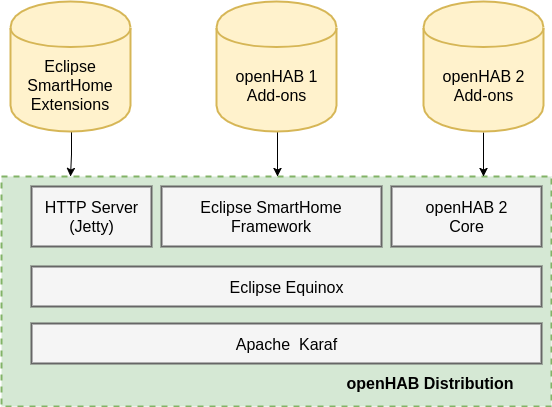
\includegraphics[width=\textwidth]{oh_architecture}
\caption{The openHAB architecture based on~\cite{openhab_02}.}
\label{fig:oh_architecture}
\end{center}
\end{figure}

\subsubsection{Eclipse SmartHome}

As the core for the openHAB software stack, Eclipse SmartHome (ESH) provides a flexible and modularized framework for smart home and ambient assisted living solutions with a focus on heterogenous environments~\cite{esh_01}. The goal of ESH is to offer a solution for the fragmented market in smart home solutions by offering a medium where vendor-incompatible devices can be operated transparently.

As in the first version of openHAB, the idea of a \emph{binding} is reused in ESH. Bindings implement a thing-specific protocol e.g.\ ZigBee, and by loading the appropriate binding, the connection between the devices or services e.g., a TV set or weather service, and the framework, can be established. Furthermore, the bindings are connected to an \emph{event bus}, and this allows to do inter-component communication. Through the event bus, it is possible to send commands to the device or service, or else to receive status updates from them.

The architecture of ESH is detailed in figure~\ref{fig:esh_architecture}. In the figure, at least four things are connected to the ESH framework through its respective bindings. There are two ways in which activity prompt changes in the things connected: through a user interface (UI) and automation logic. The UI in ESH is made up of adaptable \emph{sitemaps} comprised of dynamic web pages, and this medium allows for interaction with the things through a web browser. The automation logic is established in terms of \emph{rules}, which are specified through configuration files. Additionally, there is also a REST API which is exposed through certain URIs, not shown in this figure. For all cases, commands may be directed to the event bus, which are then forwarded to its respective binding. Likewise, status updates may be shown in the UI, or served to the automation logic to perform more operations on top of these results. Finally, it is possible to make use of a custom logging module and console, mostly for development purposes.

\begin{figure} [ht] 
\begin{center}
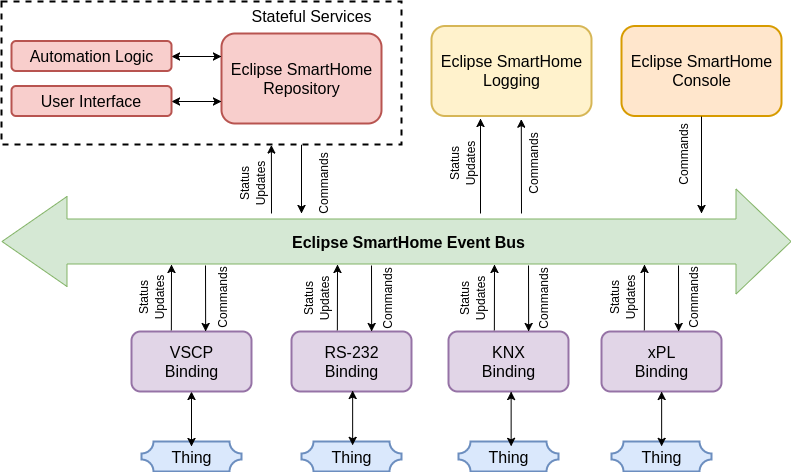
\includegraphics[width=\textwidth]{esh_architecture}
\caption{The Eclipse SmartHome architecture based on~\cite{esh_02}.}
\label{fig:esh_architecture}
\end{center}
\end{figure}

\paragraph{Summary.} This chapter had two objectives: to introduce relevant concepts about information security and the OSGi architecture used throughout the rest of this work, and to give an overview on the security challenges and threats for applications in IoT, particularly, the smart home application. Finally, it introduces two keystones for this work: Eclipse SmartHome and openHAB. Eclipse SmartHome, as the core framework of openHAB, is the focus of the contributions made in this work. An overview of the architecture of both software stacks is given in this chapter to facilitate the understanding of the architectural decisions taken later in chapter~\ref{sec:method}.

\clearpage
\section{Related Work}
\label{sec:related}
As more sensing devices capable of communication with the cloud become available to the public, more scenarios take form for the smart home. Accordingly, there is an increase of customer-ready solutions in the market. OpenHAB is but one of the existing smart home solutions. As an open-source project with a very active community, openHAB distinguises itself from other solutions. As part of the focus of this work is to review the security of openHAB, this section will look at other smart home solutions from a security and privacy perspective. 

\subsection{NEST}
NEST offers integration of NEST proprietary devices for the smart home, such as thermostats, cameras, doorbells, alarm systems, locks, smoke alarms, among others. Each of these devices are capable of connecting to a web service in the cloud. Some superficial details about the protocols and cryptographic primitives used for the device-cloud communication are disclosed, but the specifics are not published~\cite{related_01}.

The Nest apps (mobile and web), thermostats, and cameras connect to the Nest cloud service using the Transport Layer Security (TLS) protocol, and encrypt the transported data with AES-128. Particularly, the cameras use a 2048-bit RSA key when establishing the TLS session. The CO and smoke alarm devices use a proprietary protocol similar to TLS to establish the secure connection with the cloud service.

The data collected from the Nest devices is stored in Amazon Web Services and Google Cloud Platform. The privacy and security policies are enforced according to these particular third-party services~\cite{related_01}.

To control and view data from a thermostat, for example, first it has to be paired with the cloud backend. Then, by touching it (proof-of-posession) it produces a one-time password which can be entered in the mobile application. If successfully done, the client is authenticated, and only the user of this mobile application can access and control the thermostat. Additionally, this can be controlled remotely through the internet, i.e., the application connects to the cloud backend which forwards commands to the device at home.

\subsection{HomeKit}

HomeKit is a smart home solution by Apple which aims to integrate all devices of the Apple ecosystem. HomeKit uses a secure pairing mechanism to authenticate with an iDevice, e.g., iPhone, iPad, etc. It employs a propietary HomeKit Accessory Protocol (HAP) to enable third-party accessories to communicate with home or Apple devices. The HomeKit Accessory Protocol supports both IP and Bluetooth LE as transport protocol. The pairing process depends on the transport protocol: for IP, devices have to be in the same network; for bluetooth LE, pairing is peer-to-peer. Moreover, all sessions between HomeKit accessories and Apple products are mutually authenticated and encrypted~\cite{related_02}.

There is also hardware security in place. HomeKit introduced an \emph{authentication coprocessor} that only members enrolled in their MFi program can put into their accessories. A commercial HomeKit accessory must include an authentication coprocessor, and additionally include a Wi-Fi Alliance certificate or Bluetooth SIG certification, depending on the type of transport for that particular device~\cite{related_02}.

In early December 2017, a vulnerability in the Apple ecosystem, including HomeKit, allowed anyone with a valid MAC address to login as a root in the system~\cite{related_03}, without having to provide valid credentials. It was promptly patched in a security update, followed by an apology by Apple.

\subsection{OpenRemote}

OpenRemote is a flexible and open-ended solution for creating home automation environments. It is comprised of three components: an online designer software, a controller (hardware), and an app/panel front end~\cite{related_04}. In OpenRemote, no authentication is enforced by default, but it can be enabled through Apache Tomcat's configuration files. Furthermore, OpenRemote exposes a REST API which does not require authentication at all, and thus, no access control is enforced.

There was an effort to allow authentication through Public-Key Infrastructure (PKI) and transport encryption through the TLS protocol. In the proposed solution, the controller creates public-key certificates for the authorized users and acts as a certificate authority (CA). However, this solution never got integrated into the main branch of development~\cite{related_05}. 

\subsection{ThingsBoard}

ThingsBoard is a more general open-source solution for the IoT. It may be used to design solutions for smart farming, grid, telemetry, home automation, etc.~\cite{related_06}.

With respect to security, the technical documentation covers two aspects: transport encryption and device authentication. For the former, the system administrator of a ThingsBoard instance can configure it to support HTTPS connections and MQTT transports. However, DTLS for CoAP is not supported yet. For device authentication, ThingsBoard can support various types of device credentials. Current release provides support for token-based credentials for all protocols, and additionally supports X.509 certificates for the MQTT protocol~\cite{related_07}.

\subsection{The Thing System}

The Thing System is an open-source set of highly-extensible software components developed in node.js and network protocols to connect things, independent of their vendor, into a heterogenous environment~\cite{related_08}.

The Thing System enforces by default access control mechanisms, and recognizes that a single user may have more than one client (e.g.\ smart phone, laptop, tablet, etc.). If there are no users configured, the first access to the system instance may create the first user. Every time a user is created, a time-based one-time password is sent by the system. Since the process is compliant with the RFC 6238~\cite{RFC6238}, Google Authenticators and other programs may be used for web access.

Any created client may have one role out of: master, resident, guest, device, cloud. The first three roles is meant for regular users to a varying degree of permissions inside the core functionalities of The Things System. The cloud role is assigned to services accessed through the Internet, and the device role, as its name implies, is assigned to devices to be made part of the environment~\cite{related_08}. 

For the future, it is planned to implement a special sort of firewall to filter incoming traffic to the IoT environment. For this mechanism to work, the devices would need to reside on a separate network, however.

\subsection{Home Assistant}

As an open-source home automation platform created with Python 3, it aims to automate control of all devices at home in an heterogenous environment.

In terms of security, Home Assistant follows an approach of \emph{Intranet of Things} for two reasons: to maintain functionality even when an Internet connection is not available, and to keep private data from leaving the local instance~\cite{related_11}.

As part of the documentation, several guidelines are given to protect the security of Home Assistant instance, even if it is enclosed in the local area network~\cite{related_12}. These recommendations are valid for any typical web application hosted in a private network that is open to the Internet. In particular, some advice is given on how to integrate Home Assistant into the Onion network through Tor for the sake of preserving privacy on top of confidentiality. Other than this, the command line tool for Home Assistant, HASS, supports authentication for a single user. The credentials are hard-coded into the configuration files, and once a user has authenticated, it is capable of enabling IP filtering~\cite{related_10}.

\subsection{Discussion}

As the works presented in this chapter are complete solutions for home automation, they do not strictly relate to the contributions made for openHAB and Eclipse SmartHome. However, they were included in this work from a security point of view, i.e.: by giving an overview kind of the security mechanisms and access control policies defined and enforced for each of them.

In particular, Home Assistant is the one that mostly resembles openHAB in terms of functionality and security philosophy. For the sake of preserving privacy, both systems can fully operate without having an active Internet connection, thus ensuring that no data from the devices is stored in third-party servers. Since it is assumed that no unauthorized party has access to the private network, and therefore the system UI and REST API, no serious access control mechanisms are implemented. However, this is not sufficient for either because users may not be of equal standing, and some operations could be restricted for a particular user.

The access control mechanisms in The Thing System is, in part, what openHAB should strive to incorporate. With a role-based access control model, it is possible to differentiate users according to their privileges. Furthermore, by keeping profiles of devices and cloud services, it reduces the risk of spoofing. However, the authorization model implemented in The Thing System is not suitable for a escalable environment, since the quantity of things and their capabilities will only increase with time.

The current state of OpenRemote and ThingsBoard greatly resemble that of openHAB. All three support the use of encrypted connections through HTTPS, although configuration varies depending on the web server for each solution. OpenRemote could have in place a reasonable access control mechanism for its REST API if the external contribution had been adopted.

Due to their proprietary nature, HomeKit and NEST are the most distant from openHAB in terms of interoperability and design. HomeKit and Nest mandatorily require an active Internet connection at all times, and thus all data is stored in the cloud. Meanwhile, openHAB can operate out of the box without depending on access to the Internet. In terms of security, HomeKit introduces a novel hardware approach which would prevent device spoofing. In contrast, Nest provides a \emph{proof-of-posession} authentication mechanism to authenticate with the web services. Due to the specific nature of the hardware, neither solution could be implemented in openHAB.

\paragraph{Summary.} This chapter introduced six smart home applications which cover overlapping use cases, but follow distinct approaches in terms of security. Nest and HomeKit, particularly, take advantage of their hardware to enforce an additional layer of authentication and integrity protection, respectively. OpenRemote had an initiative to support public key infrastructure among peers inside the smart home ecosystem. ThingsBoard, although a more general solution for IoT, offered support for token-based credentials its compatible protocols. The Thing System incorporated a mechanism to enforce access control after the first user got registered through a time-based one-time password. Finally, Home Assistant has the capability to expose itself to Tor, thus maintaining privacy. 

\newpage
\section{Methodology}
\label{sec:method}

As a first step towards analyzing the security of IoT models, architectures, and applications, a brief study on the state of the art was conducted. From the reviewed literature, security challenges and threats in IoT were identified, along with possible countermeasures that provide data confidentiality, peer authentication, non-repudiation, etc. However, the studied proposals tended to oversimplify and deviate from the issues present in real-world, customer-ready solutions. This observation made it clear that there was a disconnect from academic publications and commercial software. Most products, however, do not make public their internal components, and tend to make their own architectural decisions instead of following standards for, e.g.\ encoding data transmitted between things. Among the existing solutions for a smart environment, the openHAB smart home software was chosen as a case study in terms of security. The decision was made for various reasons: first, it is open-source, and thus it is possible to conduct white-box testing, secondly, it is vendor-agnostic, and finally, because of the active participation of the community in this project.

\subsection{Security of openHAB}

A binding is the logical piece of the system that links a \emph{thing} to openHAB. Through the User Interface (UI) or REST API calls, a user is able to view, and possibly modify the channels, i.e.\ state values, of the things connected to the system. Temperature and humidity numbers, on/off state of light switches, information about currently playing media, etc., are some examples of these channels. In the case of the least complex adversary, it may be assumed that it is possible to eavesdrop the incoming and outgoing data packets through the network. Thus, the first effort was to see how the data is moving around the system. Through the use of Wireshark and tcpdump, it was observed that the transit of data ocurred in two possible ways: through the cloud, or through the openHAB instance. Some devices, such as light switches, do not require to communicate with a server in the Internet to set or unset the state of the switch. As this may be done internally, the binding provides the means to operate the thing directly through the User Interface of openHAB. The other case involves devices which need to communicate to a remote server through the Internet to store its data in a third-party service. The binding, in this case, connects to the remote server through a external REST API, and gets the data required from it. This is more evident in a logical thing, such as a weather service. The binding for the weather service connects to the remote server through an API to query data about temperature, humidity, etc., of a particular location.

It can be observed that there are three communication scenarios in openHAB: purely internal (thing-openHAB), external with logical thing (openHAB-remote web service), and external with physical thing (openHAB-remote web service-thing). The security implications differ in each of these scenarios.

Internal communication between things and the openHAB instance is typically done under a wireless network that encrypted with AES, for example. Because of this, an eavesdropper is only able to get the transmitted data if it can break AES, which is computationally infeasible for a sensible amount of time for even a 128-bit key. Thus, data confidentiality in this scenario depends entirely on the security of the wireless network where the openHAB instance and the thing reside. Evidently, if the attacker gains access to this private network, all intercepted communication will be plainly visible.

The second communication scenario, where the thing connects to a remote cloud server, has an additional point of vulnerability: eavesdropping and tampering within the Internet. An eavesdropper that does not have access to the private network may still find a way to obtain the data during transit after it has left the router and is moving through the Internet. Returning to the example of the weather service, a binding may be programmed to get the current temperature and humidity every 10 minutes. This e.g., HTTP request leaves the openHAB instance and goes into the router, and then it travels through distinct points along the Internet. The remote server accepts the request if valid, and returns a response with the appropriate values in a format such as JSON or XML. If this request is not encrypted (e.g., by using TLS), then the eavesdropper may easily learn the data sent back in the HTTP response.

The third scenario, communication of a thing with a remote server through openHAB was the first obstacle in the security analysis. Because of simplifications in the literature about IoT, it is typically assumed that for the architecture of IoT applications there is no connection to the Internet to accomplish a task that may be performed locally~\cite{ALABA201710}. However, due to different vendors and a variety of devices, the actual solution tends to depend on a remote connection. For this reason, the security requirements in the literature, such as in~\cite{taekim}, do not quite fit. These differences do not make the communication in openHAB inherently less secure, but in that case, the analysis should be more flexible and consider these design variations. 

This last scenario hints at the implication of guaranteeing secure communication between things, the openHAB instance, and the remote servers. Indeed, if the request performed by a binding is pointed at a location through HTTPS, then the request will perform the TLS protocol, encrypting the communication. The main question in this case is then, is it guaranteed that the request will point to an HTTPS location? The answer to this could only be found by looking at the source code of the bindings present in openHAB. Recall that through a binding, openHAB is able to send commands to things, and in this case, through the remote server.

When analyzing the source code, it becomes evident that the URL chosen to direct the request is decided at the time the binding was written. This implies that the security of each binding is independent from each other. If a binding points to a plain HTTP URL, then it is only that binding that is subject to effective eavesdropping, and it would not affect other bindings added to the system.

\newpage
\begin{lstlisting}[caption={HTTP connection for iCloud binding.},label={lst:https_binding},numbers=left,escapeinside={@}{@}]
  public class Connection {
    private final String iCloudApiURL = "https://fmipmobile.icloud.com/fmipservice/device/";
    private final String iCloudAPIRequestDataCommand = "/initClient";
    private final Gson gson = new GsonBuilder().create();
    private final String dataRequest = gson.toJson(ICloudDataRequest.defaultInstance());
    
    private final byte[] authorization;
    private URL iCloudDataRequestURL;
    
    public Connection(String appleId, String password) throws MalformedURLException {
      iCloudDataRequestURL = new URL(iCloudApiURL + appleId + iCloudAPIRequestDataCommand);
    } 
    
    public String requestDeviceStatusJSON() throws IOException {
      HttpsURLConnection connection = connect(iCloudDataRequestURL);
      String response = postRequest(connection, dataRequest);
      connection.disconnect();    
      return response;
    }
  }
\end{lstlisting}

Code snippet~\ref{lst:https_binding} is an example of a binding, in this case for the iCloud service. This binding is meant to establish a connection to the iCloud services, for example, to learn the status of a device. The method \texttt{requestDeviceStatus} is responsible for establishing the connection and returning the result as a JSON structure stored as a string. In the context of security, the important thing to note is that the connection is established through the use of the \texttt{HttpsURLConnection} class, which supports https-specific features, such as the encrypted communication through the TLS protocol~\cite{java_01}. In this case, it is expected that the communication will be encrypted, so that an eavesdropper will not be able to read the plain data.

To verify these findings, Wireshark was used to observe the packets sent from and to the openHAB instance installed in port 8090. Naturally, there were many TLS sessions packets captured in Wireshark, some of these originating from unrelated services installed in the host. One of the established sessions was for a maps web service, used in the Netatmo binding installed in this local openHAB binding. Thus, the use of Wireshark confirmed that the HTTP requests are being encrypted with TLS as defined in the corresponding bindings. Due to the privacy of the author, the captured data packets will not be disclosed. 

As hinted, the use of HTTPS in bindings is of great importance due to the underlying Transport Layer Security protocol, also known plainly as TLS. According to the specification by the IETF, TLS provides communications security over the internet, and it is designed to prevent eavesdropping, tampering, or message forgery~\cite{RFC5246}. The specifics of the protocol are of no importance in this work, thus it suffices to stress the fact that relying on it will guarantee the confidentiality and integrity of the data sent between the openHAB instance and remote servers.

\subsection{openHAB: Intranet of Things}

An openHAB instance is typically installed on a small server, even on a Raspberry Pi, deployed on some port, 8080 by default. Due to the configuration of openHAB, this port may only be accessed by end devices in the same wireless network. It has been asked by the community if it is possible to access the openHAB instance from the outside, that is: through the Internet~\cite{openhab_05}. Exposing an application to the outside may be trivial from a functional standpoint, but it carries its own set of security risks. Denial-of-Service attacks, unrestricted URL access, injection, session hijacking, etc., are only some of the possibilities that could affect an application open to the Internet. These risks are well documented by projects such as the OWASP Top Ten in IoT~\cite{owasp}. In the case of openHAB particularly, an adversary does not need to explore too much before finding out an apparent vulnerability: the lack of authentication, and therefore, absence of access control.

As mentioned in chapter~\ref{sssec:oh}, to preserve privacy it is recommended to keep the openHAB instance from being exposed to the Internet. This may satisfy a weak security requirement, but it limits the use cases for the smart home. For any smart home application it is desirable to have the possibility of secure remote access, e.g., from the office, and openHAB is no exception. For this reason, openHAB offers three options for secure remote access: VPN connection, myopenHAB Cloud Service, and running openHAB behind a reverse proxy~\cite{openhab_04}. These options have the same idea: to make the transmission channel as safe as possible to prevent any unauthorized party from entering the private network. Although these options make secure remote access viable, any adversary that gains access to the private network ends up gaining full control over openHAB. Thus, the security against adversaries is as strong as the security of the channel.

Relying purely on the communication channel makes it very difficult to make the openHAB instance securely \emph{exposed} to the Internet, even if openHAB, and not the things, is the only point of external access~\cite{openhab_03}. The main reason for this is that there is no authorization mechanism in place for alllowing or forbidding access for users. Thus, any individual that can access the openHAB instance is capable of altering the system state and retrieving any piece of data, as there is no lock in place. This threat is minimized by making the instance accessible only from inside the private network, taking the appearance of ``Intranet of Things''.  Therefore, the security of openHAB is as strong as the security of the private network. An intruder gaining access to the network implies allowing them access to all of the openHAB capabilities, thus breaching the privacy and confidentiality of the data in use.

At a first glance, one would think that authentication and access control should be implemented and managed by the final product, i.e.\ openHAB. It turns out, however, that as a core feature that involves restricting access to the REST end points and servlet extensions, it is more apropriate to fit the authentication and authorization logic inside the Eclipse SmartHome framework. Recall that Eclipse SmartHome is a subset of the openHAB distribution that holds the core functionalities for automation of sensing devices. Thus, access control, and inherently, authentication, became of interest to the Eclipse SmartHome community. 

\subsection{Community Discussion on Role-Based Access Control}
\label{ssec:discussion}

Starting from the situation that there is no access control mechanism in place, the community has long discussed the implications of implementing authentication, of any kind, and role-based access control. As the project long advanced without any foresight on access control, it has become increasingly difficult to implement any simple solution directly, as it was not in the original design. In fact, not much documentation and examples can be found for authentication and access control for OSGi-based projects, in contrast with more traditional frameworks.

One such OSGi-based project that implements authentication and access control is Apache Karaf, a container for the OSGi runtime, which provides security based on JAAS (Java Authentication and Authorization Service)~\cite{karaf}. This embdedded security system can internally control access to OSGi services, console commands, etc. This is an interesting scenario as it relies on the basic-authentication framework offered by Java, instead of relying on more heavy frameworks like Apache Shiro or Spring Security.

The community in openHAB was inspired by JAAS-based attempts at security and proposed a solution that made use of annotations and \emph{Basic} authentication. The changes of several OSGi bundles were made a pull request in eventually merged into the master branch of the project~\cite{esh_04}. First of all, the changes themselves were designed as a sort of \emph{authentication API}, rather than a unique, concrete implementation. Meaning that a good portion of the code was made up of interfaces and abstract classes that defined methods to create and manage credentials and authentication providers. A concrete implementation offered with these changes was based on the JAAS realm with \emph{Basic} authentication. Basic-authentication, in this case, means that the credentials are enclosed inside an HTTP request as a pair of the form \texttt{username:password}. These credentials are enclosed as part of the HTTP request header, and the concrete implementation is meant to extract these details from the HTTP request header to instantiate a \texttt{Credentials} object. Moreover, by relying on the JAAS realm, it was possible to use Java \emph{annotations} in the code. These annotations serve to regulate access depending on the roles that the authenticated user has. If the authenticated user has the required role, then access is granted to the method or resource. Code snippet~\ref{lst:jaas_roles} shows that to add a new thing to the openHAB environment, the role of \emph{admin} is needed. If the user is not authenticated, or has a different role, then access to the method is forbidden. 


\begin{lstlisting}[caption={Role-Based method restriction in ESH.},label={lst:jaas_roles},numbers=left]
    @POST
    @RolesAllowed({ Role.ADMIN })
    @Consumes(MediaType.APPLICATION_JSON)
    public Response create(String language, ThingDTO thingBean) {
      // Thing is added here
    }
\end{lstlisting}

There are several problems with this approach, however. First, access control is not managed through a database or any other dynamic means, but is instead static. It is defined inside the source code, and there is no way to change permissions at runtime. This means that the project would need to be built and deployed again in order to take in any changes to the authorization policy. Secondly, it offers no clear view on how the fine-grained details would have its access controlled. For example, let the status of a light bulb be of public access, but only authorized users may flip its switch from the user interface; others may only view the state of the light bulb. Moreover, a different thing could have the opposite behavior: to hide its status, but make it public to control it. As openHAB is vendor and thing-agnostic, relying on annotations makes it impossible to deal with such fine-grained details in authorization.

Following the design patterns in Apache Shiro, the authentication API for the Eclipse SmartHome was designed to have the means to plug in any authentication providers as desired. These providers may provide the authentication service either locally or remotely (e.g.\ through OAuth). The goal was to have a flexible solution that may accept different kinds of authentication mechanisms to satisfy the many different use-case scenarios. The concrete implementations would be done by the products relying on the Eclipse SmartHome, such as openHAB. Different products may have different scenarios and constraints for authentication, and so it makes sense to have some flexibility in this aspect. For example, a new user may prefer to login through their Google credentials instead of setting up a new account for the particular SmartHome instance. 

A common problem with the attempted authentication API was that there was no way to turn it off, and thus it automatically rejected all incoming requests without an authorization header~\cite{esh_05}. Normally, this is not a problem for most web applications, as there typically is a redirect method that leads to a login page, where the user can input their credentials. The authentication API, however, offered no login form, as it only supported basic-authentication out of the box. Indeed, without a way to inject the credentials into every HTTP request, the changes were mostly unusable. This was a problem especially for new users, who would have no idea on what to do whenever a ``Forbidden access'' page would come up. Originally, it was thought that if no authentication provider was available, then access control would not be enforced, making it an optional feature. However, it turned out that not detecting any authentication provider made no change whatsoever, leading to all requests to the REST end points being rejected. In the end, it was decided to disable the authentication API bundle from the default runtime, so it would not impede the normal functioning of openHAB.

From this experience, it was decided it would be desirable to have a way to \emph{turn off} access control completely, in the case that the user does not have the means to authenticate and manage permissions. At first glance, this is a very counter-intuitive feature to have, as any adversary could push toward disabling security, instead of having to break it through more advanced methods. 

As a product of the discussion at the time, the Eclipse Smarthome community created a document to define the requirements and use cases to cover the access control needs~\cite{esh_06}. An important distinction in this document was the emphasis made on the variety of \emph{resources}, and their respective implementation constraints. Resources do not only encompass \emph{things} connected to the system, but also automation rules, third-party add-ons, UI sitemaps, system settings, etc. The document delved into the management of the resources present in the system, rather than the actual security mechanisms that had to be employed. 

\subsection{Misuse Cases}

In an attempt to identify which were the aspects that more resembled requirements with respect to security, rather than management of resources, \emph{misuse cases} were written according to the state of the Eclipse Smarthome at the time. Thus, the provided requirements document included the \emph{use cases} that served as a basis to identify the \emph{misuse cases}. 

A misuse case, as the name suggests, is meant to cause the opposite consequence of a typical use case. That is, instead of designing the system to cover a certain functionality, the intention is to pinpoint which functionalities or \emph{actions} should not be permitted in the ideal system~\cite{misuse}. A misuse case diagram shows mis-actors, i.e.\ adversaries, initiating misuse cases to cause some anomaly by taking advantage of legitimate use cases.

Often, it is not obvious to identify misuse cases, as there are many angles and attack vectors that may go unnoticed to everyone but the adversary. Thus, it becomes more of a ``brainstorming'' exercise to attempt to detect possible threats, and an initial response to mitigate them. In this case, misuse cases were written to find out which threats could be posed by adversaries, and how these could be mitigated.

Figure \ref{fig:misuse_cases} shows on the left side the use cases extracted from the requirements document created from the community. Next to these, some identified misuse cases are shown to be initiated by mis-actors. The threat level of for each misuse case is not specified, as it is not entirely clear what assets have the most priority, or how easily these weaknesses could be exploited. Finally, for each of these misuse cases, a mitigation strategy is presented accordingly. It is important to stress that the purpose is not to show how these threats can be instantiated into a vulnerability, or to delve into the details of the mitigation strategy. The idea of misuse cases is to have some kind of initial understanding of threats to lead the discussion on security and further analyze it. Unfortunately, the Eclipse Smarthome community was not very interested in following up the discussion in this perspective, but preferred to focus on the more technical, hands-on, implementation of access control mechanisms to \emph{secure} resources from the automation environment.

\begin{figure} [ht] 
\begin{center}
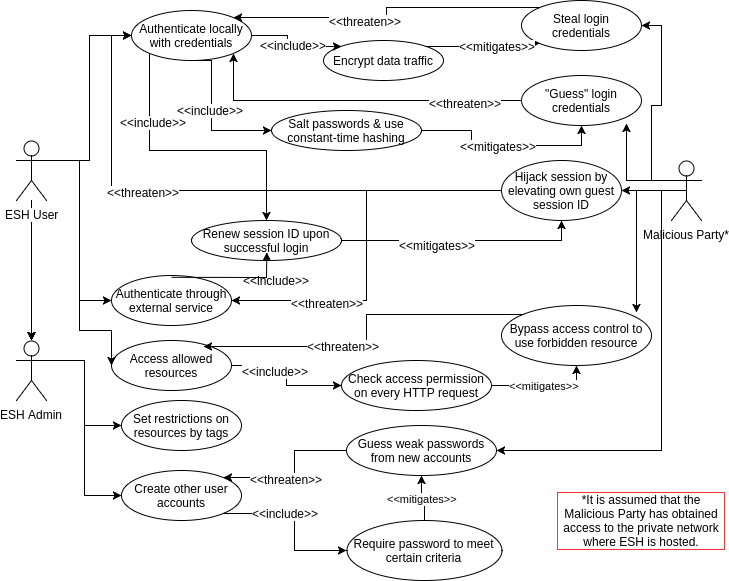
\includegraphics[width=\textwidth]{esh_misuse_cases}
\caption{Misuse Cases for Access Control in ESH.}
\label{fig:misuse_cases}
\end{center}
\end{figure}

\subsection{Proposed Token-Based Authentication Procedure}

On 15th February, 2018, a videocall meeting was held by the interested parties in the community with the purpose of clarifying the requirements gathered in the document mentioned in chapter \ref{ssec:discussion}, and set priorities accordingly. Part of the discussion also meant to address how previously attempted solutions might be of use for the future implemention of authentication and access control. Among the most relevant agreed points was the use of JSON Web Tokens (JWT) for stateless authentication. Stateless authentication inherently reduce the effort needed to manage user sesions in the backend, thus the idea was supported. It was also decided that the specifics of the access control mechanisms could be decided at a later point in time, since the most important priority was adding authentication to the Eclipse SmartHome framework. Therefore, further effort in this work was directed toward the implementation of a JWT-based authentication mechanism compatible with the Eclipse SmartHome architecture, and thus, possibly compatible also with the openHAB software stack.

Typically, all kinds of token-based authentication mechanisms follow these steps~\cite{token_auth}:
\begin{enumerate}
\item The client sends its credentials (e.g.\ username, password, fingerprint) to the server.
\item The server attempts to authenticate: if valid, it generates a token that includes expiration time.
\item The server stores a copy of the token and associates it with the user.
\item The server sends the token to the client.
\item In every future request, the client sends the token to the server.
\item For each request, the server extracts the token from the request, and looks up the user associated to it to perform authorization.
\item If the token is expired, the server generates a new token and sends it to the client. 
\end{enumerate}

The JSON Web Token (JWT) holds some peculiarities to other tokens. The primary difference is that this token includes a digital signature by the party that created it, e.g., the server. Thus, some adaptations would have to be applied to this procedure. Consider, for example, the limitations in the user interface in Eclipse SmartHome to provide web forms to put the credentials. For this reason, credentials are sent first through \emph{basic-authentication}, since the web browser takes care of asking for the credentials. Therefore, the proposed authentication mechanism is as follows:

\begin{enumerate}
\item The client sends credentials through the basic-authentication natively supported by the web browser.
\item The server extracts credentials and, if these match an existing user, it generates a JSON Web Token (JWT), appending to it the username and any additional fields, including expiration time and the server's digital signature of the JWT digest. Server sends the JWT to the client.
\item The client attaches the JWT on any future request.
\item For every request, the server extracts the JWT and verifies the digital signature. If valid, it takes the username and other claims, and performs authorization on the requested resource.
\item If the JWT is expired, the server requests credentials through basic-authentication, and if these are valid, it generates and serves a valid JWT.
\end{enumerate}

What may immediately stand out in this proposal, in contrast with the typical procedure, is the inclusion of the username as part of the fields in the JWT. Typically, a username is not considered to be \emph{confidential} and, although it normally is not made public, it gives the adversary no significant advantage on stealing a user's data. In fact, if only resource access control is the goal, then the username does not need to be included. It would be sufficient to include the claims regarding the permissions on access to the resources. Since the validity of the token is relying on the digital signature, it is guaranteed that the claims are valid. Moreover, for the sake of maintaining forward securtiy, a JWT is only renewed if the valid credentials are presented again. An adversary may, in some manner, retrieve an expired legitimate token. If this expired token would be presented to the server, then the server could present the adversary with a fresh token. Finally, as hinted, the most important distinction is the use of digital signatures within the token. Indeed, if an adversary tried to impersonate a legitimate user through guessing usernames, it would not work, as the signature would not verify on the server's end. The security of the signature is as strong as the security of the signature, which may be RSA-2048, for instance. 

The aforementioned procedure was designed with the assumption that, at all times, an HTTPS connection is present and thus, communication is protected through the TLS protocol. Otherwise, credentials and JWTs could be intercepted at any time by an adversary. A digital signature does not offer data confidentiality, after all.

\subsection{Architectural Implications of Authentication}

As a multi-layered automation software solution, it is not trivial to implement authentication, no matter the type, so that all parts of the system are covered by it. Recall that in chapter \ref{ssec:discussion} it was stated that resources in the smart home ecosystem do not only involve things, but also many different aspects of the system. Moreover, the Eclipse Smarthome is designed according to the OSGi architecture, and thus all modules are maintained as \emph{bundles}. These bundles contain, among other things, typical Java servlets and REST endpoints. If the methods present inside these Java classes have to go through some kind of \emph{check} before being executed, then access control may be implemented. This chapter gives details on the architecture and current development affairs, but this is introduced only as a base to delve into the proposed solution for authentication with JWT.

The idea, in general, is that any incoming HTTP request would have to be caught before running whatever Java method it attempted to access. For typical OSGi applications, the use of \emph{filters} is most commonly encouraged. A filter is a mechanism that may be applied before or after a Java method is accessed. Thus, it becomes a natural choice to employ filters for the purpose of access control.

It turns out, however, that regular filters do not work for the methods involving REST endpoints, such as a GET operation to return a list of all connected devices. These methods are actually based on the JAX-RS specification for a REST API in Java. In short, they require a different type of filters, which use a set of classes different from the regular OSGi filters. Aditionally, to make use of JAX-RS in OSGi applications, it is needed to use a third-party connector. Previous work on authentication for the Eclipse SmartHome made use of this connector and the special filters. There were problems with using these special filters, however: first of all, the role permissions could only be set within the code, thus it was not a good mechanism for managing permissions at a more granular scale; secondly, due to classloading problems, it is a problem in some scenarios to make use of the JAX-RS third-party connector; and finally, this special filter is not compatible with traditional servlets (i.e., those that do not involve the JAX-RS REST API).

As part of the OSGi release 6 specification, filters may be registered to any resource through a special mechanism called the ``whiteboard pattern''. Current implementation of the Eclipse SmartHome runtime is bounded by the OSGi~4.2 specification, and due to constraints in the rest of the software stack, it is not immediately feasible to update the runtime to a newer specification. Part of the work by the community was to create a \emph{bridge} between the OSGi~4.2 runtime and the newer whiteboard pattern functionality. For some time, this work attempted to implement JWT authentication for a ficticious, patched runtime that supported the use of the filters registered by the whiteboard. However, it was later decided that this bridge was not trivial, and the community halted its development.

As this particular development of the Eclipse Smarthome halted, a new direction involving traditional servlet security was considered for this work. As part of servlet registration to the OSGi runtime, an entity called \texttt{HttpContext} has to be provided. This entity provides the means to intercept HTTP requests before they reach the servlet, and thus it becomes the point where authentication and authorization may be implemented. Originally, this approach was discarded because the REST endpoints did not support the use of a \texttt{HttpContext} shared with the other servlets. The key in this case is that both groups of servlets, the traditional and the REST servlet, run under different application contexts. What this means is that, even if a traditional servlet handles authentication properly, this information would not be propagated to the REST endpoints, and thus authorization mechanisms would not be enforced. In the months of March and April, however, part of the community started an effort to combine, or rather, to \emph{bridge} the provided \texttt{HttpContext} among servlets and REST endpoints, virtually creating a single application context for all servlets.

Figure~\ref{fig:esh_auth_arch} shows at a very high level the underlying architecture of the Eclipse SmartHome runtime. At the lowest level, the Jetty HTTP server and servlet engine is running. On top of it, there are several servlets running separately. Part of these servlets may be associated as being \emph{traditional}, while a particular servlet, the REST servlet, runs under different conditions. The REST servlet is used to serve resources, typically in the form of JSON structures, that contain data about things, items, channels, etc. The Chart and Icon servlets are more traditional servlets and thus, run under the same shared application context. Meanwhile, the REST servlet is shown to run under an isolated application context. Thus, the solution worked on by the community is to \textbf{bridge} both application contexts and therefore have a commonly shared \texttt{HttpContext}~\cite{esh_03}. Yellow boxes represent the entities or resources that should have its access restricted according to a specified policy. Green boxes represent the possible solution to the problem, whereas the red boxes are the attempted solutions in previous years. Particularly, ``JAX-RS Custom ContainerContext'' was an attempted solution by the community, which had many problems when ported into the final openHAB software stack. An alternative solution to it, the ``JAX-RS Custom Filter'' was originally planned to be implemented for this work, but the notion was discarded after understanding the limitations of this kind of filter, since it would not enforce authorization for the rest of the servlets (e.g.\ Icon servlet). 

\begin{figure} [ht] 
\begin{center}
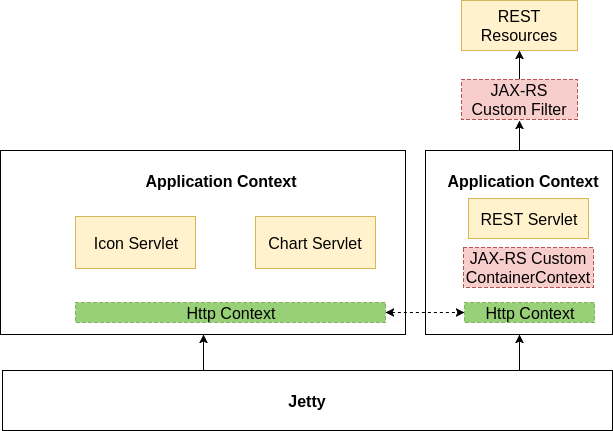
\includegraphics[width=0.8\textwidth]{esh_auth_arch}
\caption{Architecture breakdown into servlets.}
\label{fig:esh_auth_arch}
\end{center}
\end{figure}

Initial results by the community~\cite{esh_03} showed that it was indeed possible to make the \texttt{HttpContext} shared by the components that needed access control. Taking these results into account, work in the direction of a \emph{custom} \texttt{HttpContext} started. For this, the merged \texttt{HttpContext} requires the existence of an authenticator, i.e.\ a module that performs the authentication logic, and thereafter the module that performs authorization. Figure~\ref{fig:esh_arch_authenticator} shows how the authenticator is merely a black box performs the logic of a certain type of authentication, such as the basic or token-based. The decision is based on the received HTTP request: depending on whether it has a session identifier (e.g.\ cookie), an authorization header, or neither. And if it does have one of these, to which authenticator the credentials would be directed to. Implementation details for the basic and JWT authenticators are introduced in chapter~\ref{ssec:impl}. Form authentication is left as future work. 

\begin{figure} [ht] 
\begin{center}
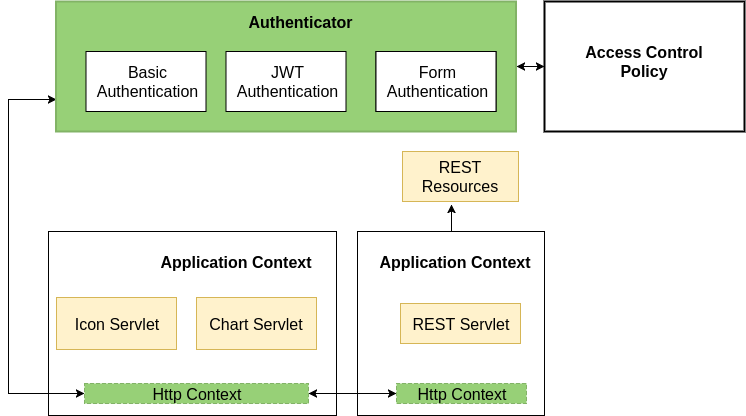
\includegraphics[width=0.8\textwidth]{esh_arch_authenticator}
\caption{Addition of authenticators into the architecture.}
\label{fig:esh_arch_authenticator}
\end{center}
\end{figure}

After the process of authentication, what follows is authorization. The authorization itself depends on the access control policies decided for each particular resource and the privilege level of the user requesting access. This work focuses on authentication, and thus does not include the implementation of a particular access control policy. However, a proposal for access control is made in chapter~\ref{ssec:autho}.

\subsection{Implementation of Authenticators}
\label{ssec:impl}

To model the sequence of events ocurring during the intended authentication procedure, a sequence diagram was written and is shown in figure~\ref{fig:esh_auth_sequence}. This diagram shows the most compelling scenario: where the client interacts the first time with a servlet to get access to a resource. Clearly, as no credentials are provided at this time, the servlet demands basic-authentication, and from the received valid credentials it generates a JSON Web Token (JWT). This token is reused in all subsequent requests by the client. Note that the authorization policy is not included into this sequence of events. Thus, authorization becomes a binary aspect: if credentials are valid, then access is granted to the resource, regardless of its nature. Due to simplification, this diagram is only considering the use of valid credentials. In the actual implementation, invalid credentials result in a ``Forbidden Access'' response. 

\begin{figure} [ht] 
\begin{center}
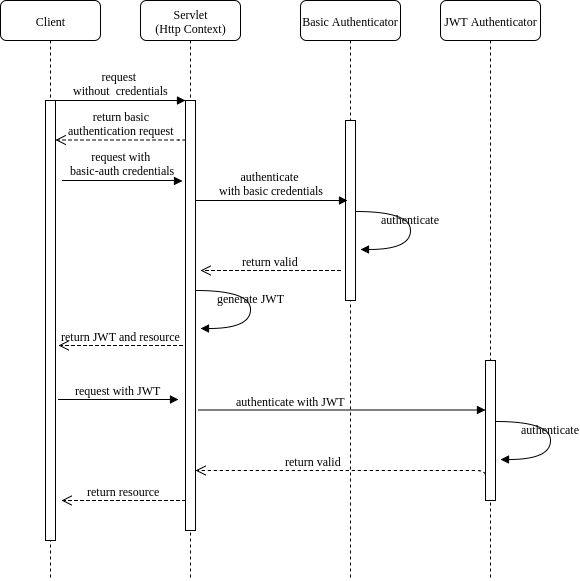
\includegraphics[width=0.8\textwidth]{esh_auth_sequence}
\caption{Authentication sequence diagram.}
\label{fig:esh_auth_sequence}
\end{center}
\end{figure}

The implementation of the authenticators was made into the \texttt{auth} bundle of the Eclipse SmartHome framework. Due to the hierarchical nature of this project, many details will be omitted. The core of the authenticator is located as part of the \texttt{CustomHttpContext} code located in this bundle.

As an interface class of the \texttt{Http Service} OSGi feature, \texttt{HttpContext} includes a method \texttt{handleSecurity} which, as the name implies, handles the security for the specified request to the servlet. As long as the servlet is registered with the custom \texttt{HttpContext}, every request into the servlet will go through the \texttt{handleSecurity} method.

\begin{lstlisting}[caption={Core implementation of \texttt{CustomHttpContext}.},label={lst:core_impl},numbers=left,escapeinside={@}{@}]    
class CustomHttpContext implements HttpContext {   
 boolean handleSecurity(request,response) {
  if(request.getHeader("Authorization") == null \
       && request.getHeader("Cookie") == null) {
    response.addHeader("WWW@-@Authenticate", \
	"Basic realm=\"Test Realm\"");
    response.sendError(HttpServletResponse.SC_UNAUTHORIZED;
    return false;
  }	    
  if(jwtAuthenticated(request)) {
    return true;		
  } else if(basicAuthenticated(request)){
    username = getUsername(request);
    freshToken = generateJwt(username);
    response.addHeader("Set@-@Cookie", freshToken);
    return true;
  } else {
    response.sendError(HttpServletResponse.SC_UNAUTHORIZED);
    return false;
  }
 }
}
\end{lstlisting}

The simplified code snippet shows the core part of the \texttt{HttpContext} that intercepts requests and performs authentication from the provided HTTP header. As shown in the code snippet, after the JWT has been generated, it is given to the client as a \emph{cookie}. This way, no logic has to be implemented to manage token storage in the client side (e.g.\ through local storage using HTML5). In subsequent requests, the cookie is presented to the server, and from it, the token is extracted and verified.

To handle the creation and verification of a JWT, a third-party library, Nimbus, was used~\cite{nimbus}. This library also provides more complex features such as encryption of the JWT via symmetric key encryption. These features are not currently considered for this work. As part of the basic structure of the JWT, a signature from the host is included at the end of the claims (e.g., username, permissions). For the proof of concept, an RSA-1024 key is generated as a singleton during runtime. Using the singleton pattern ensures that multiple private keys do not exist simultaneously, which would cause conflicts during signature verification. The freshly created RSA key is then used to both generate and sign the JWT, as shown in the simplified code snippet~\ref{lst:rsa}.

\begin{lstlisting}[caption={Generation and signing of the JWT.},label={lst:rsa},numbers=left,escapeinside={@}{@}]
    
  protected String generateJwt(String username, String claim) {
    RSAPublicKey publicKey = (RSAPublicKey)getKeyPair().getPublic();
    RSAPrivateKey privKey = (RSAPrivateKey)getKeyPair().getPrivate();
    JWSObject jwsObject = new JWSObject(
    new JWSHeader.Builder(JWSAlgorithm.RS256).keyID("123").build(),
    new Payload(username));
    jwsObject.sign(new RSASSASigner(privKey));
    return jwsObject.serialize();	
  }    
\end{lstlisting}

Code for the verification of the JWT is omitted as it follows a very similar logic to JWT generation and signing, but in reverse order. This implies de-serializing the JWT, loading the RSA public key into some object, verifying JWT using said object, and finally extracting username and any other claims. In the implementation, the username need not be extracted, as it is guaranteed that the claims are valid, given that the signature is valid.

As mentioned, the RSA key is generated once at runtime. Originally, this was merely be a placeholder for a pre-existing RSA key that is already present in the distribution of openHAB. This RSA key is used by openHAB for SSH access. This pre-existing RSA key is stored in a file \texttt{keys.properties} under the \texttt{etc/} directory of the installation path of openHAB. However, it turned out that some problems emerged from this idea. First, the pre-existing RSA key was disabled, i.e.\ commented, as a security precaution. Secondly, the key is only enabled after running the Karaf console inside the openHAB distribution. As Karaf is not included within the Eclipse SmartHome distribution, there is no pre-existing key. For the first problem, it would be enough to have the openHAB administrator generate a fresh key pair and store the public and private keys. However, this is not exactly user-friendly, and thus becomes a problem in terms of security usability. A solution to the overall problem is to leave key generation to the \texttt{auth} bundle and store it in some file in the local filesystem. When the bundle is activated it will first look for the file before attempting to generate a new RSA key. As the discussion within the community has not gotten to this point, the implementation has maintained the idea of storing the RSA key in memory during runtime. It should not cause problems and, in case that the bundle is restarted, then due to invalid JWTs, credentials will be requested again.

The rest of the implementation follows the logic for the basic and token-based authentication mechanisms. The code is currently maintained as two independent repositories: one that uses the whiteboard pattern~\cite{repo_02}, and one as a fork of the Eclipse SmartHome project~\cite{repo_01}. The latter does not include the JWT authenticator logic due to problems described in chapter~\ref{sec:eval}.
  
\subsection{Proposed Authorization Model}
\label{ssec:autho}

An access control system is typically split up in several phases: defining a security policy, selecting an authorization model, implementing the model, and enforcing the policy~\cite{access_01}. As a smart home automation software, it is not trivial to define a security policy that covers all scenarios, due to the dynamic and multi-purpose devices present. The implementation of any authorization model emcompasses engineering work tightly related to the architecture of the system (in this case, the OSGi framework), and thus, is left out of the scope of this work. However, by acknowledging which the resources need to be restricted through access control, e.g.\ things, items, channels, system settings; an authorization model can be proposed independently of the authorization policy and implementation. Then, when a specific policy is decided by the Eclipse SmartHome community, the model will not change drastically, and thus, implementation can follow. 

For a smart home application, the focus of an authorization model should lean towards privacy-preservation and usability~\cite{access_01}. Considering that most end users of the openHAB are not tech-savvy, some options for an authorization model are instantly discarded. Some models are considered to be too complex to manage and set up, such as the Attribute-Based Acess Control (ABAC), Usage Control (UCON), and the Access Control Matrix and List (ACM, ACL).

According to the requirements document written by the Eclipse Smart Home community, fine-grained access control is desirable~\cite{esh_06}. This is, a user with high-level privileges should be allowed to manage things-related permissions for each registered user, along with any permissions for sitemaps (User Interface templates), system settings, and others. A fine-grained authorization model that is capable of satisfying these requirements is the Attribute-Based Access Control (ABAC) model. This model, however leaves a lot to be desired in terms of usability due to the management of every single permission as attributes for every user. This kind of management might end up in user pains, opting users to disable access control for the sake of comfort. 

Initially, it was considered to make direct use of the Role-Based Access Control (RBAC) authorization model. However, this kind of model works best when there are role differences between the users of the system. In the case of openHAB, all users are typically members of the same household or temporal guests. In that sense, it does not make much sense to have a role separation between users. However, it is reasonable to assume that some members of the household may not have the same rights as others to the devices. For example, a guest could be allowed to turn on/off the light switch, but may not be allowed to freely open the front door anytime. Likewise, permissions might not be equally split even among the permanent residents.

It was observed that the difference between users depended not on roles, but rather on the capabilities owned by each subject. The Capability-Based Access Control (CapBAC) overlaps with the idea of dynamically managing capabilities by granting some kind of token that describes these capabilities~\cite{access_01}. At first, it seems that this idea better fits as an authorization model for openHAB due to the flexibility to define permissions according to the capabilities of an entity. This notion is disolved when the implications of CapBAC are further analyzed, however. The authorization that CapBAC seeks to enforce is continous, that is, authorization is checked before, during, and afterward access to a resource is requested. This particularity is meant to serve for the dynamic nature of the general IoT environment. However, for openHAB, a smart home application, the dynamic nature of smart devices is bounded by the application itself: a single home.

A fine-grained, yet usable authorization model that makes use of the concept of roles as in the RBAC model and that focuses on capabilities, is described as follows. Consider a set of activities or tasks that may be performed on the Eclipse SmartHome, and consequently, the openHAB distribution. These tasks may vary from viewing or changing the status of a device connected to the system, to accessing certain parts of the sitemaps that serve as the user interface templates. These tasks may be grouped together as capability sets. For instance, the capability set ``speakers-playback'' may include actions such as modifying the speakers volume and even stopping or changing the track currently playing. Meanwhile, the capability set ``speakers-quiet'' may allow access to viewing the track currently playing and decreasing the speakers volume, for example. Consider a collection of different capability sets designed in advance for every \emph{type} of thing, usually encompassed by a \emph{binding} in the Eclipse SmartHome. Finally, every user may be assigned a different collection of capability sets, thus preserving the idea that users may not have equal rights in the smart ecosystem. In that sense, a set of capabilities is akin to the concept of role in the RBAC model, and every user is assigned one or more roles, according to the actions permitted to them.

Table~\ref{tbl:autho_cap} shows a sample assignment of capability sets to some users. Every user is expected to have at least one capability set, which may inherently encompass a number of permissions for the system. Table~\ref{tbl:autho_op} offers an example that details the operations that access would be permitted for a particular capability set. For instance, a user with the \emph{things-all} capability set would have access to the REST resource that returns a JSON of all added things, as well as access to the method that allows registering a new thing to the ecosystem. Thus, the proposed authorization model inspired by both the RBAC and CapBAC is a sound solution for the access management needs required of the Eclipse SmartHome and openHAB automation ecosystem. 

\begin{table}[h]
  \centering
  \begin{tabular}{|l|l|}
    \hline
    \multicolumn{1}{|c|}{\textbf{User}} & \multicolumn{1}{c|}{\textbf{Capability Sets}}            \\ \hline
    Marian                              & (speakers-quiet, lights-on, doors-close, sitemaps-paper) \\ \hline
    Erika                               & (speakers-playback, lights-all, doors-all, sitemaps-all) \\ \hline
  \end{tabular}
  \caption{Sample relation of user and capability sets}
  \label{tbl:autho_cap}
\end{table}

\begin{table}[h]
  \centering
  \begin{tabular}{ll}
    \hline
    \multicolumn{1}{|c|}{\textbf{Capability Set}} & \multicolumn{1}{c|}{\textbf{Involved Operations}}                                                                                                                                                                                      \\ \hline
    \multicolumn{1}{|l|}{speakers-playback}   & \multicolumn{1}{l|}{\begin{tabular}[c]{@{}l@{}}yamahareceiver.internal.state.\\NavigationControlState.getCurrentItemName()\\ ZoneControlState.volume\end{tabular}} \\ \hline
    \multicolumn{1}{|l|}{things-all}          & \multicolumn{1}{l|}{\begin{tabular}[c]{@{}l@{}}rest.core.internal.thing.ThingResource.getAll()\\ rest.core.internal.thing.ThingResource.create()\end{tabular}}                       \\ \hline
    &
  \end{tabular}
  \caption{Sample listings of operations involved for each capability set}
  \label{tbl:autho_op}
\end{table}

The proposed authorization model fulfills the purpose noted at the beginning of this chapter: satisfying security usability and fine-grained access control. Through the assignation of capability sets, users are capable of setting the permissions without troubling themselves with complex configuration options. Moreover, through the definition of the operations involved in a capability set, the developer of a particular binding or component of Eclipse SmartHome or openHAB is able to implement the access control policy.

\paragraph{Summary.} This chapter showed in detail the heart of the contributions made in this work for Eclipse SmartHome and consequently, openHAB. First, the security of openHAB was analyzed at a communication level between things, the openHAB instance, and remote REST APIs. Then, openHAB design decisions about ``Intranet of Things'' were discussed. Later, the long-time held community discussion about authentication and access control was introduced, and its points were summarized. As an important contribution to securing openHAB, a JWT authenticator was implemented in Java according to the OSGi architecture. Finally, a fine-grained, yet usable authorization model that uses the concept of capability sets was proposed for the smart home ecosystem.

\newpage
\section{Evaluation}
\label{sec:eval}

As one of the main contributions for this work, the basic and JSON Web Token-based authenticators were implemented as a bundle for the OSGi runtime used in Eclipse SmartHome (ESH). This chapter looks at the resulting authentication bundle and how it is used alongside the other bundles for the ESH distribution. Recall that the ESH framework is a core component for the openHAB automation software. Thus, if the solution does not work in ESH, it will not work on openHAB.

The first successful attempt at implementing the authenticators was made outside the ESH ecosystem~\cite{repo_02}. Instead of relying on the Equinox OSGi runtime~4.2 that ESH is based on, the deployment was made for Apache Karaf~4.2, which supports up to the specification of OSGi~6. This implementation included an activator of the bundle, a servlet, and a custom \texttt{HttpContext} to intercept the HTTP request. The goal is to have a servlet published as an HTTP service in the OSGi runtime. However, any request to this servlet is intercepted by the \texttt{handleSecurity} method of the custom \texttt{HttpContext}, which decides if the request goes through or not. In this case, it contained the logic for basic and JWT authentication. This implementation was first built with Maven using \texttt{\$ mvn clean install}, and then deployed to Apache Karaf as a stand-alone bundle with \texttt{\$ install -s mvn:org.dreamland./org.dreamland.whitefilter/1.0.0-SNAPSHOT}. Inside Karaf, executing \texttt{http:list} showed that the installed bundle exposed an HTTP service published in the \texttt{/whitefiltered} path, which represented the resource servlet to be secured.

Accessing the servlet resource through e.g.\ curl, without any credentials, gets a response: ``HTTP ERROR 401. Problem accessing /whitefiltered. Reason: Unauthorized''. Passing the hard-coded, valid credentials by adding the \texttt{-u} parameter to curl gets a \texttt{200 OK} response from the web server. If the servlet was accessed from a web browser, then the server returns a cookie alongside the response. This cookie, a very long string, is where the JSON Web Token is stored. In subsequent HTTP requests, the cookie is sent to the server to perform JWT authentication. The response by the servlet does not change, however, so by observing the Karaf log in the \texttt{/system/console/log} it can be confirmed that the JWT authentication worked flawlessly. JWT revokation due to expiration is not implemented, and therefore the same token may be reused as long as the same RSA key is being used by the server to verify the signature of the JWT.

The next step in the evaluation of the implementation was to relocate the authentication logic into the core bundles of the Eclipse SmartHome. Very similar steps were followed, except that the bundle was built from the package \texttt{org.eclipse.smarthome.auth\\.jwt}. First, the logic for basic-authentication was put into a custom \texttt{HttpContext} as before. A test resource servlet was also included in this bundle. The activator, however, used the \texttt{HttpService} and \texttt{ServiceTracker} to register the servlet and custom context as an HTTP service in the OSGi runtime. For the previous deployment, the registration was made under the whiteboard pattern supported by OSGi 6 implementations.

Up to the experimentation of the basic-authentication, everything was replicated exactly under the ESH environment. However, when attempting to include the third-party library, Nimbus, problems started to arise. Particularly, a persistent class-loading problem for this library could not be solved, not even with the support of a very active developer of the Eclipse SmartHome and openHAB. The exact error is as follows: \texttt{Missing constraint: Import-Package: com.nimbusds.jose}, which suggests that the JAR file is not recognized by the runtime. The usual approach for including third-party libraries into a bundle for ESH is to create a \texttt{lib} directory in the root of the bundle, and put the respective JAR there. Then, the \texttt{build.properties} and \texttt{MANIFEST.MF} files have to be changed to load the classes from the JAR. This same approach has been followed in other bundles in the ESH distribution, such as the \texttt{org.eclipse.smarthome.model.persistence} bundle. However, not even replicating the same structure as this other bundle made it possible to recognize the Nimbus JAR.

Essentially, the implementation of the basic and JWT authenticators was successfully deployed into the OSGi runtime in Karaf. The testing of the deployment showed no flaws when initiating HTTP requests via curl or the web browser. The deployment of the basic authenticator for the OSGi runtime in ESH was succesfully replicated. It effectively prevent unauthorized access to a servlet resource. However, the deployment of the JWT authenticator for ESH ran into class-loading problems, and thus its effective functioning could not be verified.

\paragraph{Summary.} In essence, the proposed implementation of basic and JWT authenticators for the ESH ecosystem was evaluated in two steps. A stand-alone, OSGi-based ecosystem running in Karaf was used as the first step of evaluation. As this was an independent deployment, there were no class-loading issues with the third-party library used for JWT verification, Nimbus. The JWT and basic authenticators worked as proposed in this deployment. The second stage of evaluation was made within the ESH ecosystem. In this deployment, class-loading issues were found within ESH that impeded the use of Nimbus. Thus, only the basic authenticator for securing servlet resources could be successfully tested in this environment.

\newpage
\section{Conclusion and Future Research Directions}
\label{sec:conclusion}
This work gave an overview of the security challenges present in applications for Internet of Things, particularly in the domain of smart homes. It analyzed the security mechanisms employed in openHAB and Eclipse SmartHome, especially in terms of access control and privacy. Upon observing the lack of authentication and authorization mechanisms, a JSON Web Token-based authenticator was implemented according to the principles of the OSGi framework. An additional basic authenticator was also implemented as a fallback mechanism in case the client cannot store a JSON Web Token as a cookie. Finally, a fine-grained, yet usable authorization model was proposed for Eclipse SmartHome and openHAB. This authorization model distinguishes between users who may have overlapping permissions, but should not have equal control among all resources of the smart home ecosystem.

\subsection{Contributions}

As one of the main contributions, a custom \texttt{HttpContext} was successfully implemented to intercept all incoming requests toward the registered resource servlet. Depending on the value returned by the \texttt{handleSecurity} method, access to a resource was either allowed or forbidden. Based on this behavior, the authentication logic via a JSON Web Token was implemented within the aforementioned method. In the evaluation of this first step, JWT authentication was successfully enforced for all client requests to the servlet: clients with an invalid token, or with no token at all were denied access to the servlet resource. As the second step of the implementation, a secondary \emph{basic} authenticator was implemented which demanded credentials from the client's web browser as a prompt. The evaluation was performed in two stages. The first stage was made outside the ESH runtime, in an isolated OSGi environment, under Karaf as container. Both the basic and JWT authenticators were effectively able to authenticate incoming HTTP requests to the servlet. First time clients were always asked for credentials to authenticate, and then further requests transitioned into the JWT authentication. Thus, only when the client provided either valid basic credentials or JWT, access to the servlet resource was allowed. The second stage of the evaluation made use of the same authentication logic, but deployed under the ESH OSGi runtime. Due to class-loading problems, the JWT authenticator was not able to be tested. However, the basic authenticator, which did not depend on external libraries, effectively restricted access to the servlet resource if the credentials were not provided in the header of the HTTP request.

The second contribution for Eclipse SmartHome and openHAB was the proposal of a fine-grained, yet usable authorization model. This model was inspired by the RBAC and CapAC models, and adjusted accordingly to fit within the smart home paradigm. Most importantly, the concept of \emph{capability sets} is used to encompass resources and functionalities of the smart home ecosystem. Users get assigned capability sets to reflect an access control policy that maps the authority of a user to specific capabilities of the smart home ecosystem. A capability set could be defined as part of the definition of a binding, for example.

\subsection{Future Research Directions}

There are several endeavors in terms of implementation that may be considered for future work. The most apparent one is related to the class-loading problems in Eclipse SmartHome that impede the use of a third-party library for JWT generation and verification. Otherwise, it could also be considered to implement a JWT generator and verifier using the tools provided by the native Java API.

Furthermore, for the sake of usability, it could be considered to implement a form-based authentication mechanism compatible with the implemented authenticators. After all, due to the architecture of Eclipse SmartHome, it is not trivial to plug-in a redirect from every resource to a web form for authentication.

In terms of JWT management and forward-security, it would be desirable to have an expiration date for the generated JSON Web Tokens. For this, a renewal procedure should be implemented. If the token has already expired, then credentials would be requested once again through an encrypted transport (e.g.., HTTPS). Additionally, it could also be considered to encrypt the JWT according to the specification, for the sake of adding another layer of confidentiality protection.

Furthermore, it could be considered how an RSA key can be obtained before the authenticators are called for JWT generation and verification. An option could be to generate the key pair during deployment of ESH or openHAB. 

Regarding the overall architecture of ESH, it is still not clear how to make use of the authenticator for the REST API. At the time of writing, the \emph{bridge} of \texttt{HttpContext} between the two kinds of servlets (traditional and REST) has not been made in the development branch of Eclipse SmartHome, and thus experimentation is not yet possible.

As the authenticators were implemented as black boxes, a proper user management database or filesystem is not yet in place. It is of interest how existing solutions for storage of user profiles e.g., LDAP, relational databases, could be adapted into the OSGi architecture for ESH.

A long existing problem for the ESH community regarding turning \emph{off} access control should also be considered in solutions intended for production. Creating a backdoor in to bypass security is never a good idea, after all. Instead, it could be considered that access control is enabled for the first time after a user has been created. Thus, there would be always at least one user that satifies the security policy. 

A concrete definition and implementation of the mechanisms based on the proposed authorization model. Finally, a fresh re-evaluation of the access control mechanisms could be carried out.

Finally, this work looked at the scenario of authentication \emph{within} the ecosystem, but as Internet of Things, there are other authentication scenarios. By employing OAuth, for example, a user may choose to through e.g., Google, Facebook, Twitter, etc, expanding the use cases and options for users.

\paragraph{Summary.} This chapter finalizes this work by giving some final remarks on the contributions proposed for securing openHAB and Eclipse SmartHome through user authentication and authorization. In terms of authentication, basic and JWT authenticators were implemented according to the OSGi framework. For authorization, a model inspired on RBAC and CapBAC was proposed with fine-grained access control and usability in mind. Following up from this work, several future research directions may be considered. Future work may encompass further implementation efforts on the authenticators, both local and remote; design and implementation of local management of users (e.g., through LDAP), and setting up access control after registration of the first user. Moreover, a concrete authorization implementation based on the proposed model could be explored. 

\newpage

% BibTeX bibliography
\bibliographystyle{plain}%alpha} %plain=[1], alpha=[BGZ09]
\bibliography{master-thesis}

\addcontentsline{toc}{section}{\refname}


% Use Biblatex if you have problems with Estonian keywords
%\printbibliography %biblatex

\newpage
%\appendix
%\section*{\appendixname}
\iflanguage{english}%
  {\section*{Appendix}
  \addcontentsline{toc}{section}{Appendix}
  }%
  {\section*{Lisad}
  \addcontentsline{toc}{section}{Lisad}}
  
%% \section*{I. Glossary}
%% \addcontentsline{toc}{subsection}{I. Glossary}
%% \TODO{FINISH GLOSSARY}
%% Bearer token. The digest of the user credentials to be used in an authentication process.
%% Manifest. Configuration file for OSGi bundles that define the bundle's unique identification, packages imported from other bundles, and packages to make available to other bundles.
%% IP. Internet Protocol.
  %% CoAP.
  %TLS
  % DTLS
  
%% HTTPS.
%% MQTT.
%% Spoofing.
%% curl.
%% JAR.
%% Thing.
%% Eclipse SmartHome
%\newpage

%=== Licence in English
\newcommand\EngLicence{{%
\selectlanguage{english}
\section*{I. Licence}

\addcontentsline{toc}{subsection}{I. Licence}

\subsection*{Non-exclusive licence to reproduce thesis and make thesis public}

I, \textbf{Jes\'{u}s Antonio Soto Vel\'{a}zquez},

\begin{enumerate}
\item
herewith grant the University of Tartu a free permit (non-exclusive licence) to:
\begin{enumerate}
\item[1.1]
reproduce, for the purpose of preservation and making available to the public, including for addition to the DSpace digital archives until expiry of the term of validity of the copyright, and
\item[1.2]
make available to the public via the web environment of the University of Tartu, including via the DSpace digital archives until expiry of the term of validity of the copyright,
\end{enumerate}

of my thesis
\textbf{Securing openHAB Smart Home through User Authentication and Authorization}

supervised by Satish Narayana Srirama and Danilo Gligoroski

\item
I am aware of the fact that the author retains these rights.
\item
I certify that granting the non-exclusive licence does not infringe the intellectual property rights or rights arising from the Personal Data Protection Act. 
\end{enumerate}

\noindent
Tartu, 21.05.2018
}}%\newcommand\EngLicence


%=== Licence in Estonian
\newcommand\EstLicence{{%
\selectlanguage{estonian}
\section*{II. Litsents}

\addcontentsline{toc}{subsection}{II. Litsents}

\subsection*{Lihtlitsents lõputöö reprodutseerimiseks ja lõputöö üldsusele kättesaadavaks tegemiseks}

Mina, \textbf{Jes\'{u}s Antonio Soto Vel\'{a}zquez},

\begin{enumerate}
\item
annan Tartu Ülikoolile tasuta loa (lihtlitsentsi) enda loodud teose

\textbf{Tüübituletus neljandat järku loogikavalemitele}

mille juhendajad on Satish Narayana Srirama ja Danilo Gligoroski

\begin{enumerate}
\item[1.1]
reprodutseerimiseks säilitamise ja üldsusele kättesaadavaks tegemise eesmärgil, sealhulgas digitaalarhiivi DSpace-is lisamise eesmärgil kuni autoriõiguse kehtivuse tähtaja lõppemiseni;
\item[1.2]
üldsusele kättesaadavaks tegemiseks Tartu Ülikooli veebikeskkonna kaudu, sealhulgas digitaalarhiivi DSpace´i kaudu kuni autoriõiguse kehtivuse tähtaja lõppemiseni.
\end{enumerate}


\item
olen teadlik, et punktis 1 nimetatud õigused jäävad alles ka autorile.
\item
kinnitan, et lihtlitsentsi andmisega ei rikuta teiste isikute intellektuaalomandi ega isikuandmete kaitse seadusest tulenevaid õigusi. 
\end{enumerate}

\noindent
Tartus, 21.05.2018
}}%\newcommand\EstLicence


%===Choose the licence in active language
\iflanguage{english}{\EngLicence}{\EstLicence}


\end{document}

